% =====================================================================
%  Road to RoboCup -- main file
%  Compile with:  pdflatex main.tex   (run twice for the table of contents)
%
%  Things you may want to change:
%    \BookTitle, \BookSubtitle, \BookTagline, \BookAuthor   (title page)
%    \answermode   back | inline | off                      (answers)
%  Chapters live in  chapters/<part>/<chapter>/chapter.tex  and answers.tex
% =====================================================================
\documentclass[11pt,a4paper,twoside]{book}

% ---------------- Title page texts ----------------
\newcommand{\BookTitle}{Road to RoboCup}
\newcommand{\BookSubtitle}{The Math Behind Neural Networks and\\ Soccer-Playing Robots\\[0.2em]--- Starting from the Basics}
\newcommand{\BookTagline}{A course for future RoboCup champions}
\newcommand{\BookAuthor}{Stella Alice Schlotter}

% ---------------- Answers: back | inline | off ----------------
%  back   = all answers collected in an appendix at the end of the book
%  inline = answers printed at the end of each chapter
%  off    = no answers (e.g. for a student version of a test)
\newcommand{\answermode}{back}

% ---------------- Packages ----------------
\usepackage[utf8]{inputenc}
\usepackage[T1]{fontenc}
\usepackage{mathpazo}
\usepackage[scaled=0.92]{helvet}
\usepackage{microtype}
\usepackage{amsmath,amssymb,amsthm}
\usepackage[a4paper,inner=2.8cm,outer=2.3cm,top=2.6cm,bottom=2.6cm]{geometry}
\usepackage{enumitem}
\usepackage[most]{tcolorbox}
\usepackage{xcolor}
\usepackage{tikz}
\usetikzlibrary{arrows.meta,positioning,calc}
\usepackage{pgfplots}
\usepgfplotslibrary{groupplots}
\pgfplotsset{compat=1.18}
\usepackage{etoolbox}
\usepackage{array}
\usepackage{subcaption}
\usepackage{graphicx}
\graphicspath{{images/}}
\usepackage{url}
\usepackage{fancyhdr}
\usepackage{titlesec}
\usepackage[hidelinks]{hyperref}

\setlength{\parindent}{0pt}
\setlength{\parskip}{0.6em}
\setcounter{tocdepth}{0}
\setcounter{secnumdepth}{1}

% ---------------- Colours ----------------
\definecolor{cupnavy}{RGB}{8,24,56}
\definecolor{cupgold}{RGB}{232,177,52}
\definecolor{cuppitch}{RGB}{18,110,60}
\definecolor{cupred}{RGB}{200,30,40}

% ---------------- Boxes and environments ----------------
\newtcolorbox{keyidea}[1][Key idea]{colback=blue!5,colframe=blue!60!black,fonttitle=\bfseries,title=#1}
\newtcolorbox{aibox}[1][Link to AI and robotics]{colback=green!5,colframe=green!40!black,fonttitle=\bfseries,title=#1}
\newtcolorbox{stepbox}[1]{colback=orange!6,colframe=orange!60!black,fonttitle=\bfseries,title=#1}

\theoremstyle{definition}
\newtheorem{definition}{Definition}[chapter]
\newtheorem{example}{Example}[chapter]

% ---------------- Math macros ----------------
\newcommand{\R}{\mathbb{R}}
\newcommand{\sig}{\sigma}
\newcommand{\dd}{\mathrm{d}}
\newcommand{\der}[2]{\dfrac{\dd #1}{\dd #2}}
\newcommand{\pder}[2]{\dfrac{\partial #1}{\partial #2}}
\newcommand{\vv}[1]{\mathbf{#1}}
\newcommand{\norm}[1]{\left\lVert#1\right\rVert}

% ---------------- Plot styles ----------------
% gr  : with axis labels x and y     grn : without axis labels
\pgfplotsset{
  gr/.style={
    width=7.2cm, height=6cm, axis lines=middle,
    xlabel={$x$}, ylabel={$y$}, grid=both,
    grid style={line width=0.1pt, draw=gray!30},
    major grid style={line width=0.2pt, draw=gray!50},
    tick label style={font=\footnotesize},
    legend style={font=\footnotesize, fill=white, fill opacity=0.85, draw=gray!50, text opacity=1},
    every axis plot/.append style={thick}, samples=100, enlargelimits=false
  },
  grn/.style={
    width=7.2cm, height=6cm, axis lines=middle, grid=both,
    grid style={line width=0.1pt, draw=gray!30},
    major grid style={line width=0.2pt, draw=gray!50},
    tick label style={font=\footnotesize},
    legend style={font=\footnotesize, fill=white, fill opacity=0.85, draw=gray!50, text opacity=1},
    every axis plot/.append style={thick}, samples=100, enlargelimits=false
  }
}

% ---------------- Chapter, part and section style ----------------
\titleformat{\chapter}[display]
  {\sffamily\bfseries}
  {\color{cupnavy}\fontsize{54}{54}\selectfont\thechapter\vspace{-0.2em}\color{cupgold}\rule{4cm}{2.5pt}}
  {0.6em}
  {\color{cupnavy}\Huge}
\titlespacing*{\chapter}{0pt}{-10pt}{26pt}
\titleformat{name=\chapter,numberless}[display]
  {\sffamily\bfseries}{}{0pt}{\color{cupnavy}\Huge}
\titleformat{\section}{\sffamily\Large\bfseries\color{cupnavy}}{\thesection}{0.8em}{}
\titleformat{name=\section,numberless}{\sffamily\large\bfseries\color{cupnavy}}{}{0pt}{}
\titlespacing*{\section}{0pt}{1.6em}{0.5em}
\titleformat{\subsection}{\sffamily\bfseries\color{cupnavy}}{\thesubsection}{0.8em}{}
\titleformat{name=\subsection,numberless}{\sffamily\bfseries\color{cupnavy}}{}{0pt}{}

\titleformat{\part}[display]
  {\sffamily\bfseries\centering}
  {\color{cupgold}\Large\MakeUppercase{Part}\ \thepart}
  {1em}{\color{cupnavy}\fontsize{30}{36}\selectfont}

% ---------------- Headers and footers ----------------
\newcommand{\currentchaptertitle}{}
\newcommand{\bookchapter}[1]{\chapter{#1}\gdef\currentchaptertitle{#1}}
\pagestyle{fancy}
\fancyhf{}
\renewcommand{\headrulewidth}{0.4pt}
\fancyhead[LE]{\sffamily\small\thepage\quad\textcolor{cupnavy}{\BookTitle}}
\fancyhead[RO]{\sffamily\small\nouppercase{\leftmark}\quad\thepage}
\fancypagestyle{plain}{\fancyhf{}\renewcommand{\headrulewidth}{0pt}\fancyfoot[C]{\sffamily\small\thepage}}

\makeatletter
\def\cleardoublepage{\clearpage\if@twoside\ifodd\c@page\else\hbox{}\thispagestyle{empty}\newpage\fi\fi}
\makeatother

% ---------------- Answer handling ----------------
\makeatletter
\newcommand{\collectedanswers}{}
\newcommand{\ansnum}{\thechapter}
\newcommand{\answerentry}[3]{%
  \renewcommand{\ansnum}{#1}%
  \section*{Chapter #1: #2}%
  \input{#3}%
}
\newcommand{\registeranswers}[1]{%
  \ifdefstring{\answermode}{inline}{%
    \section*{Answers to the practice problems}%
    \renewcommand{\ansnum}{\thechapter}%
    \input{#1}%
  }{%
    \ifdefstring{\answermode}{back}{%
      \protected@edef\@tmp@ans{\noexpand\answerentry{\thechapter}{\currentchaptertitle}{#1}}%
      \expandafter\g@addto@macro\expandafter\collectedanswers\expandafter{\@tmp@ans}%
    }{}%
  }%
}
\makeatother
\newcommand{\block}[1]{\addtocontents{toc}{\protect\par\protect\addvspace{3pt}\protect\noindent{\protect\sffamily\protect\small\protect\color{cupgold}\protect\textbf{#1}}\protect\par\protect\nopagebreak[4]}}
\newcommand{\includeplanned}[1]{\input{chapters/#1/chapter}}
\newcommand{\includechapter}[1]{%
  \input{chapters/#1/chapter}%
  \registeranswers{chapters/#1/answers}%
}

% ---------------- Title page ----------------
\newcommand{\makebooktitle}{%
\begin{titlepage}
\thispagestyle{empty}
\begin{tikzpicture}[remember picture,overlay]
  % background
  \fill[cupnavy] (current page.south west) rectangle (current page.north east);
  % pitch at the bottom
  \shade[top color=cupnavy, bottom color=cuppitch]
    ([yshift=1cm]current page.south west) rectangle ([yshift=8cm]current page.south east);
  \fill[cuppitch] (current page.south west) rectangle ([yshift=1cm]current page.south east);
  \begin{scope}
    \clip (current page.south west) rectangle ([yshift=8cm]current page.south east);
    \draw[white,opacity=0.28,line width=1.6pt] ([yshift=1.6cm]current page.south west) -- ([yshift=1.6cm]current page.south east);
    \draw[white,opacity=0.28,line width=1.6pt] ([yshift=1.6cm]current page.south) circle (3.2cm);
    \draw[white,opacity=0.28,line width=1.6pt] ([yshift=-2.5cm]current page.south) circle (6.5cm);
  \end{scope}
  % gold accent line
  \fill[cupgold] ([xshift=2cm,yshift=-3.2cm]current page.north west) rectangle ++(1.6cm,0.12cm);
  % texts
  \node[anchor=north west,text width=11cm,align=left,text=cupgold,font=\sffamily\bfseries\small]
    at ([xshift=2cm,yshift=-3.6cm]current page.north west) {\MakeUppercase{\BookTagline}};
  \node[anchor=north west,text width=13cm,align=left,text=white,font=\sffamily\bfseries\fontsize{58}{60}\selectfont]
    at ([xshift=2cm,yshift=-4.6cm]current page.north west) {\BookTitle};
  \node[anchor=north west,text width=10.5cm,align=left,text=white,font=\sffamily\Large]
    at ([xshift=2cm,yshift=-9.4cm]current page.north west) {\BookSubtitle};
  % robot
  \node[anchor=south east,inner sep=0pt]
    at ([xshift=-0.9cm,yshift=1.0cm]current page.south east)
    {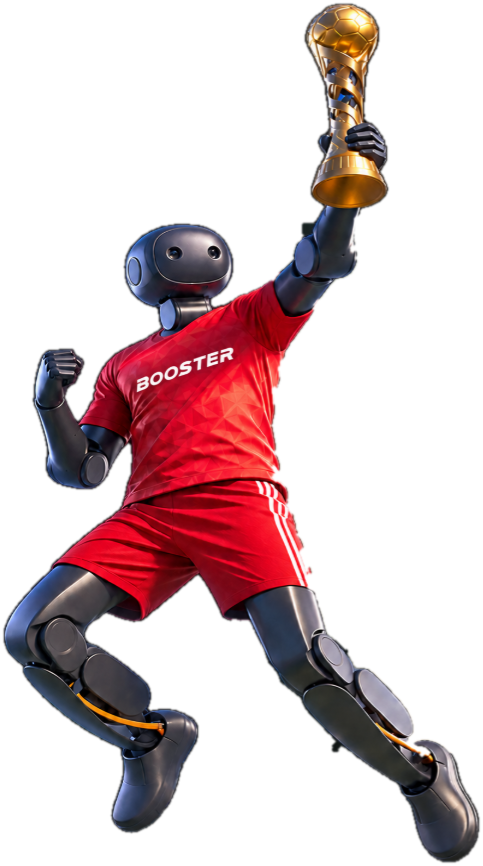
\includegraphics[height=18.5cm]{images/robot.png}};
  % author
  \node[anchor=south west,text=white,font=\sffamily\large,align=left]
    at ([xshift=2cm,yshift=1.2cm]current page.south west) {\BookAuthor};
\end{tikzpicture}
\end{titlepage}
}

\title{\BookTitle}
\author{\BookAuthor}
\date{}

\begin{document}

\frontmatter
\makebooktitle
\cleardoublepage
\tableofcontents

\chapter*{How to use this book}
\markboth{How to use this book}{How to use this book}
\addcontentsline{toc}{chapter}{How to use this book}

This book takes you from the first graph you ever drew to a neural network that learns by itself, and shows on the way why robots, and in particular soccer-playing robots as in the RoboCup competition, need exactly this mathematics.

\textbf{Structure.} The book has twelve parts. Each chapter has a short explanation, worked examples, figures and (in the written chapters) practice problems. Chapters that are marked \emph{Planned content} are not written yet.
\begin{enumerate}[nosep,label=\textbf{Part~\Roman*:},leftmargin=4.2em]
  \item \textbf{Mathematical Foundations:} functions, geometry, vectors and matrices, calculus, a tiny neural network, probability.
  \item \textbf{Linux:} the operating system of the robot and of your laptop.
  \item \textbf{Python Programming.}
  \item \textbf{Hardware:} computers, networks, sensors, microphones and motors.
  \item \textbf{ROS 2:} the software framework of the robot.
  \item \textbf{Artificial Intelligence:} tasks, data, vision models and YOLO, language models.
  \item \textbf{Reinforcement Learning.}
  \item \textbf{Rust Programming.}
  \item \textbf{Motions for the Booster K1:} simulation, training and deployment.
  \item \textbf{Control, State Estimation and Perception:} balance, filters, localisation.
  \item \textbf{RoboCup:} rules, team play, engineering practice and reliability.
  \item \textbf{Bonus: Video Analysis.}
\end{enumerate}

\textbf{Boxes.} A \emph{Key idea} box (blue) summarises the most important rule of a section. A \emph{Link to AI and robotics} box (green) shows where the topic is used later in the book.

\textbf{Problems.} Problems are numbered by chapter, so \textbf{7.3} is the third problem of Chapter~7. Problems marked with $\star$ are harder, and problems marked with \texttt{[code]} are best solved on a computer.

\textbf{Answers.} \ifdefstring{\answermode}{back}{Answers to all problems are collected at the end of the book.}{\ifdefstring{\answermode}{inline}{Answers follow at the end of each chapter.}{This version of the book does not contain answers.}}

\textbf{Suggested route.} Read the parts in order. If you already know a topic, skim its chapter and jump straight to the practice problems: if you can solve them, move on.

\chapter*{Motivation: Why Robots Need Math}
\markboth{Motivation}{Motivation}
\addcontentsline{toc}{chapter}{Motivation: Why Robots Need Math}

\section*{A flip that looks easy}
Look at the pictures below. A humanoid robot, the Booster K1, jumps, rotates backwards through the air and lands on its feet again: a \emph{webster flip}. A human gymnast needs years of training for a move like this. A robot has to do it with motors, sensors and a program, and every single frame of the motion is decided by mathematics.

\begin{figure}[htbp]
	\centering
	\begin{subfigure}[b]{0.19\textwidth}
		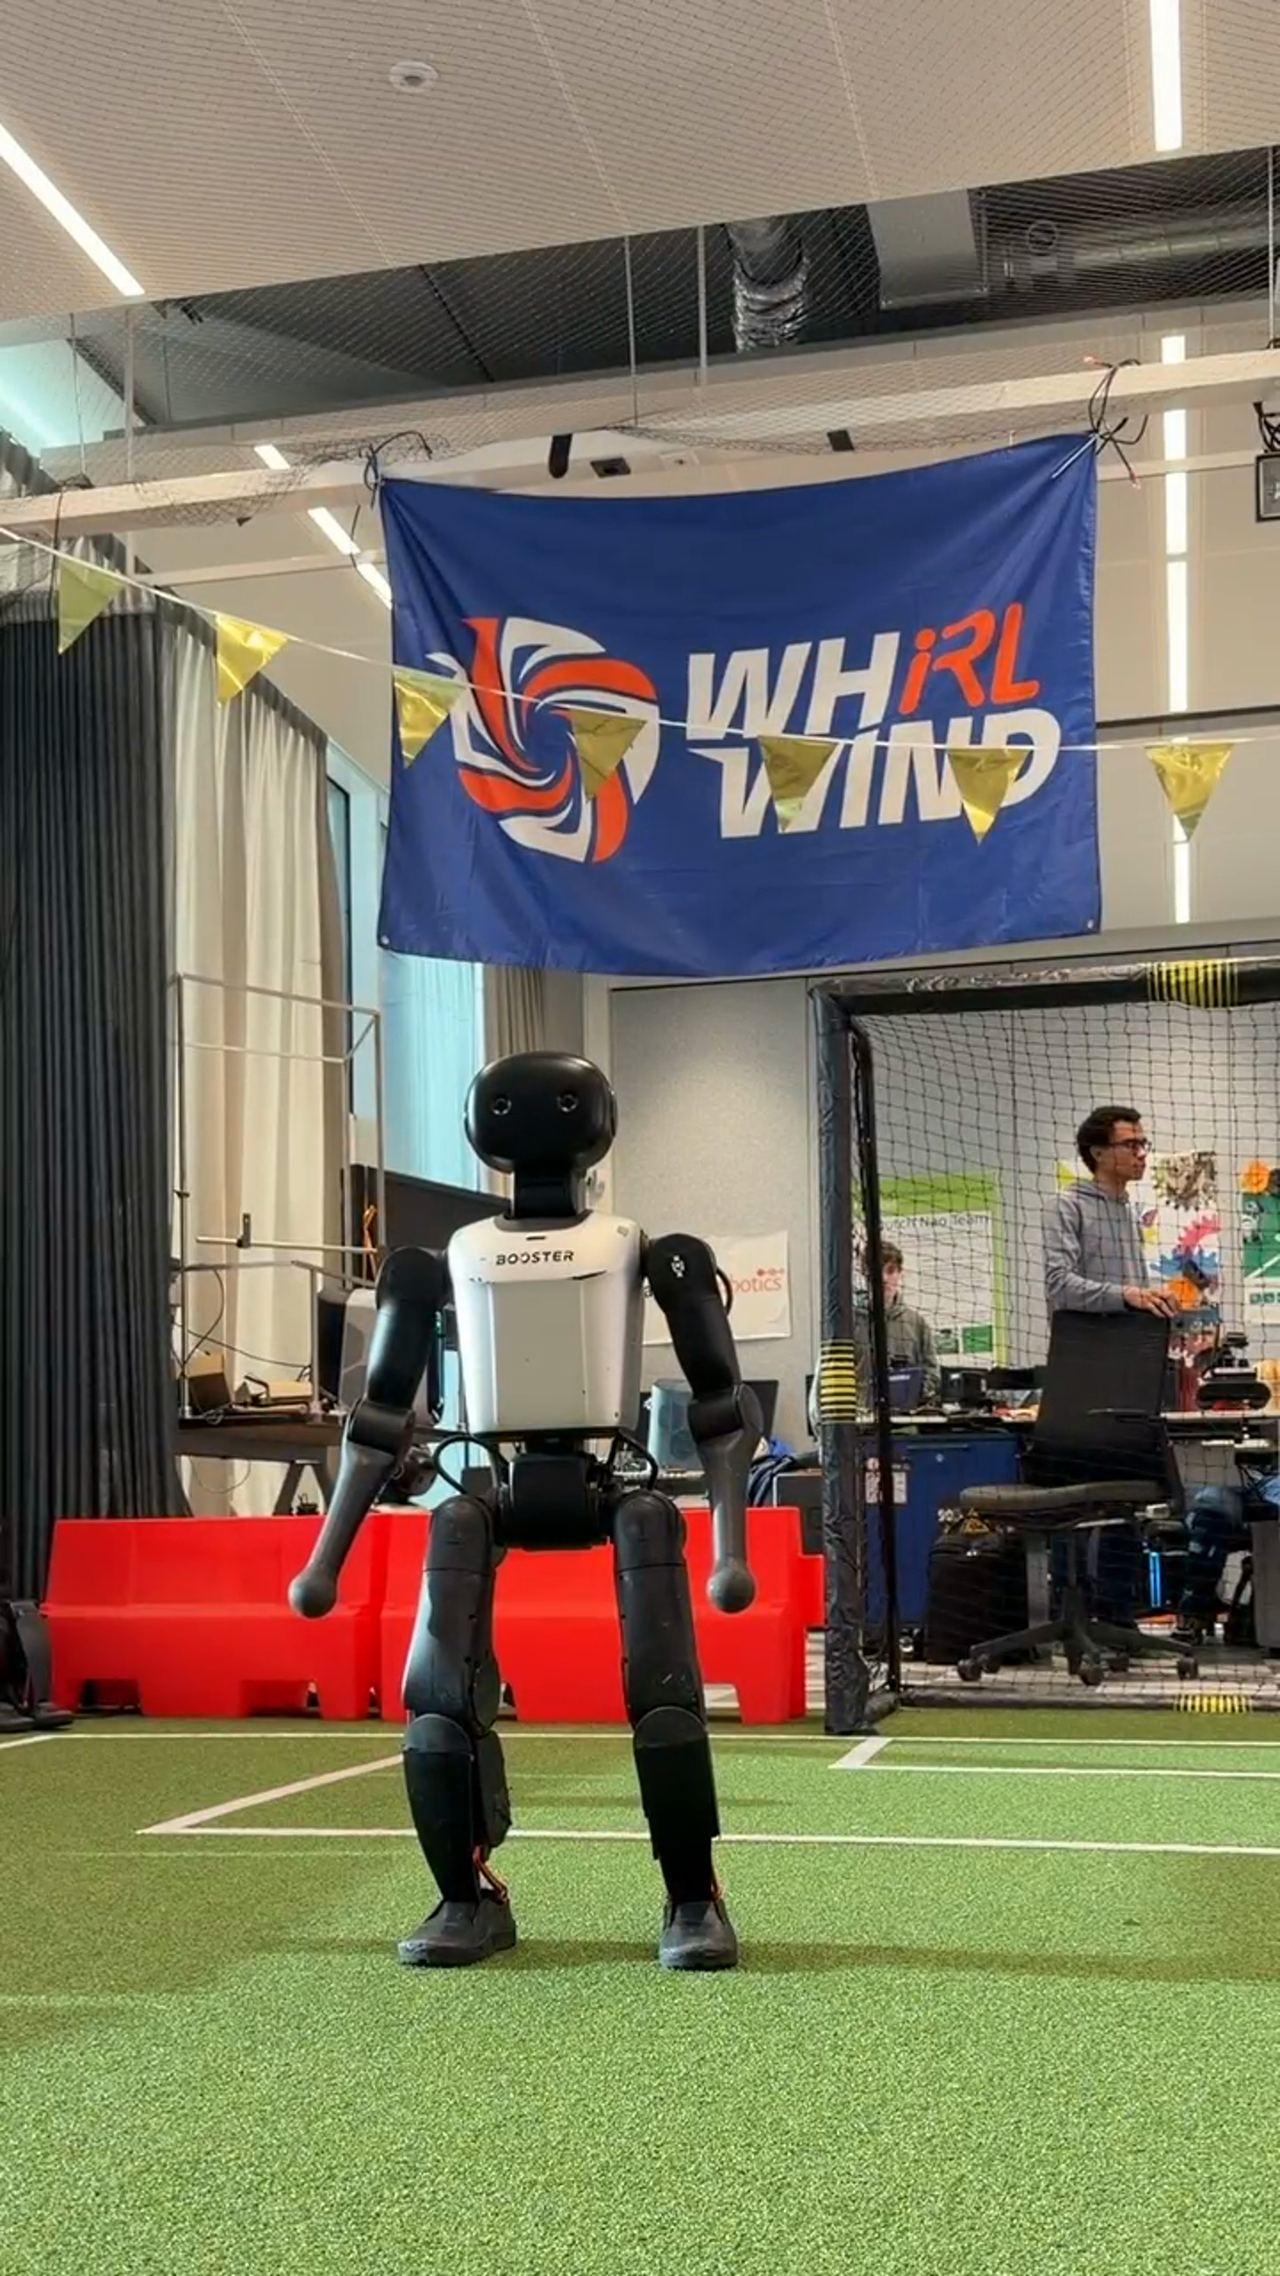
\includegraphics[width=\linewidth]{webster_flip/01.png}
	\end{subfigure}\hfill
	\begin{subfigure}[b]{0.19\textwidth}
		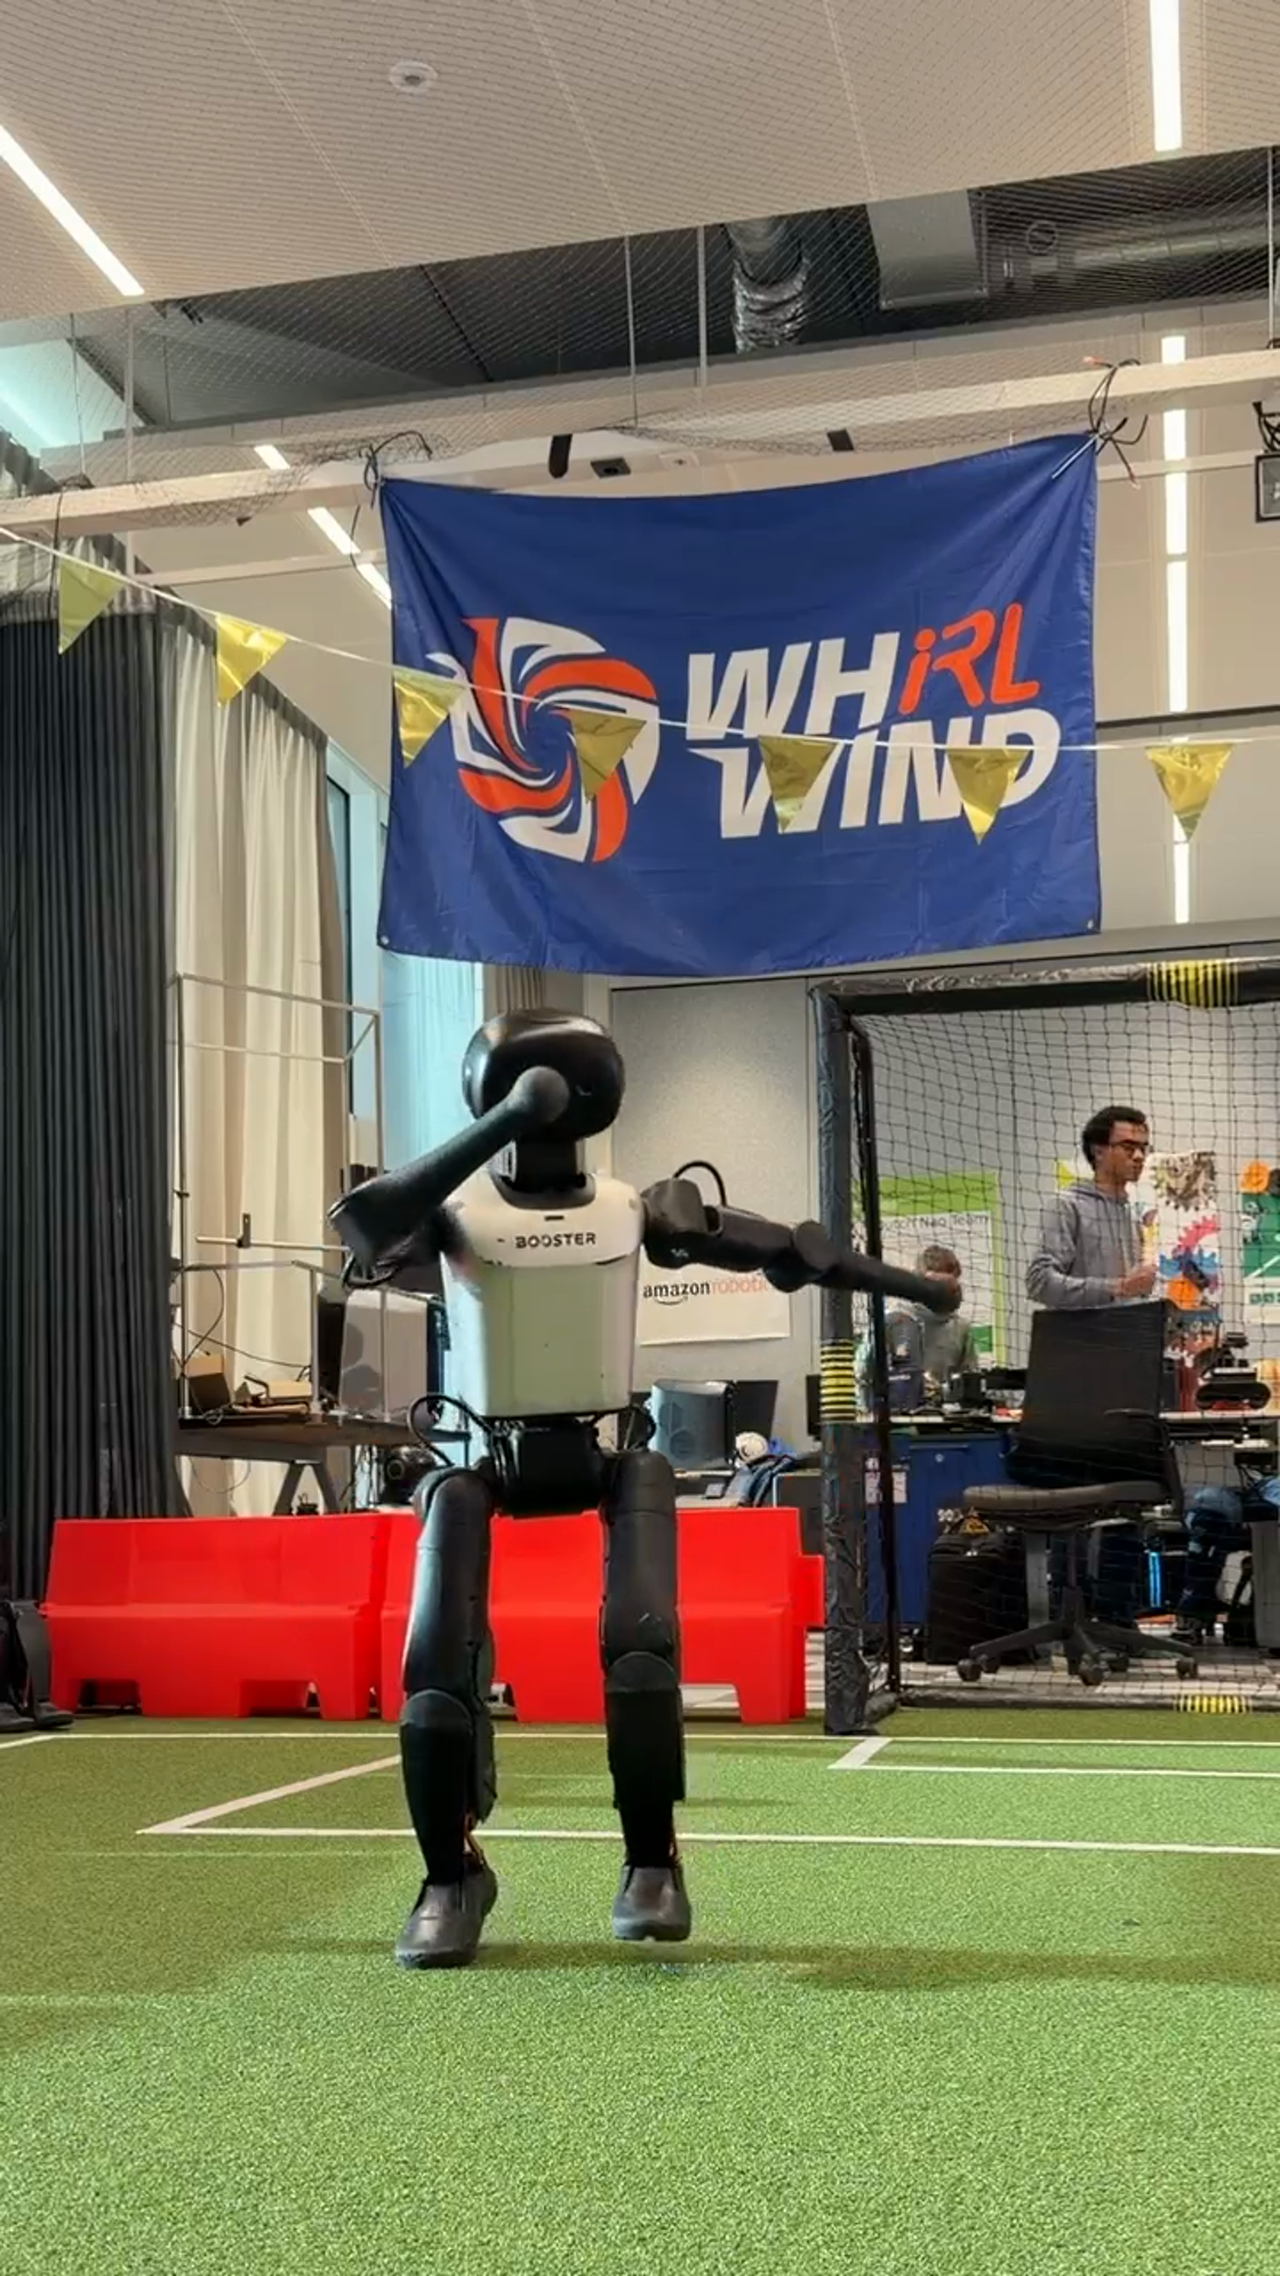
\includegraphics[width=\linewidth]{webster_flip/02.png}
	\end{subfigure}\hfill
	\begin{subfigure}[b]{0.19\textwidth}
		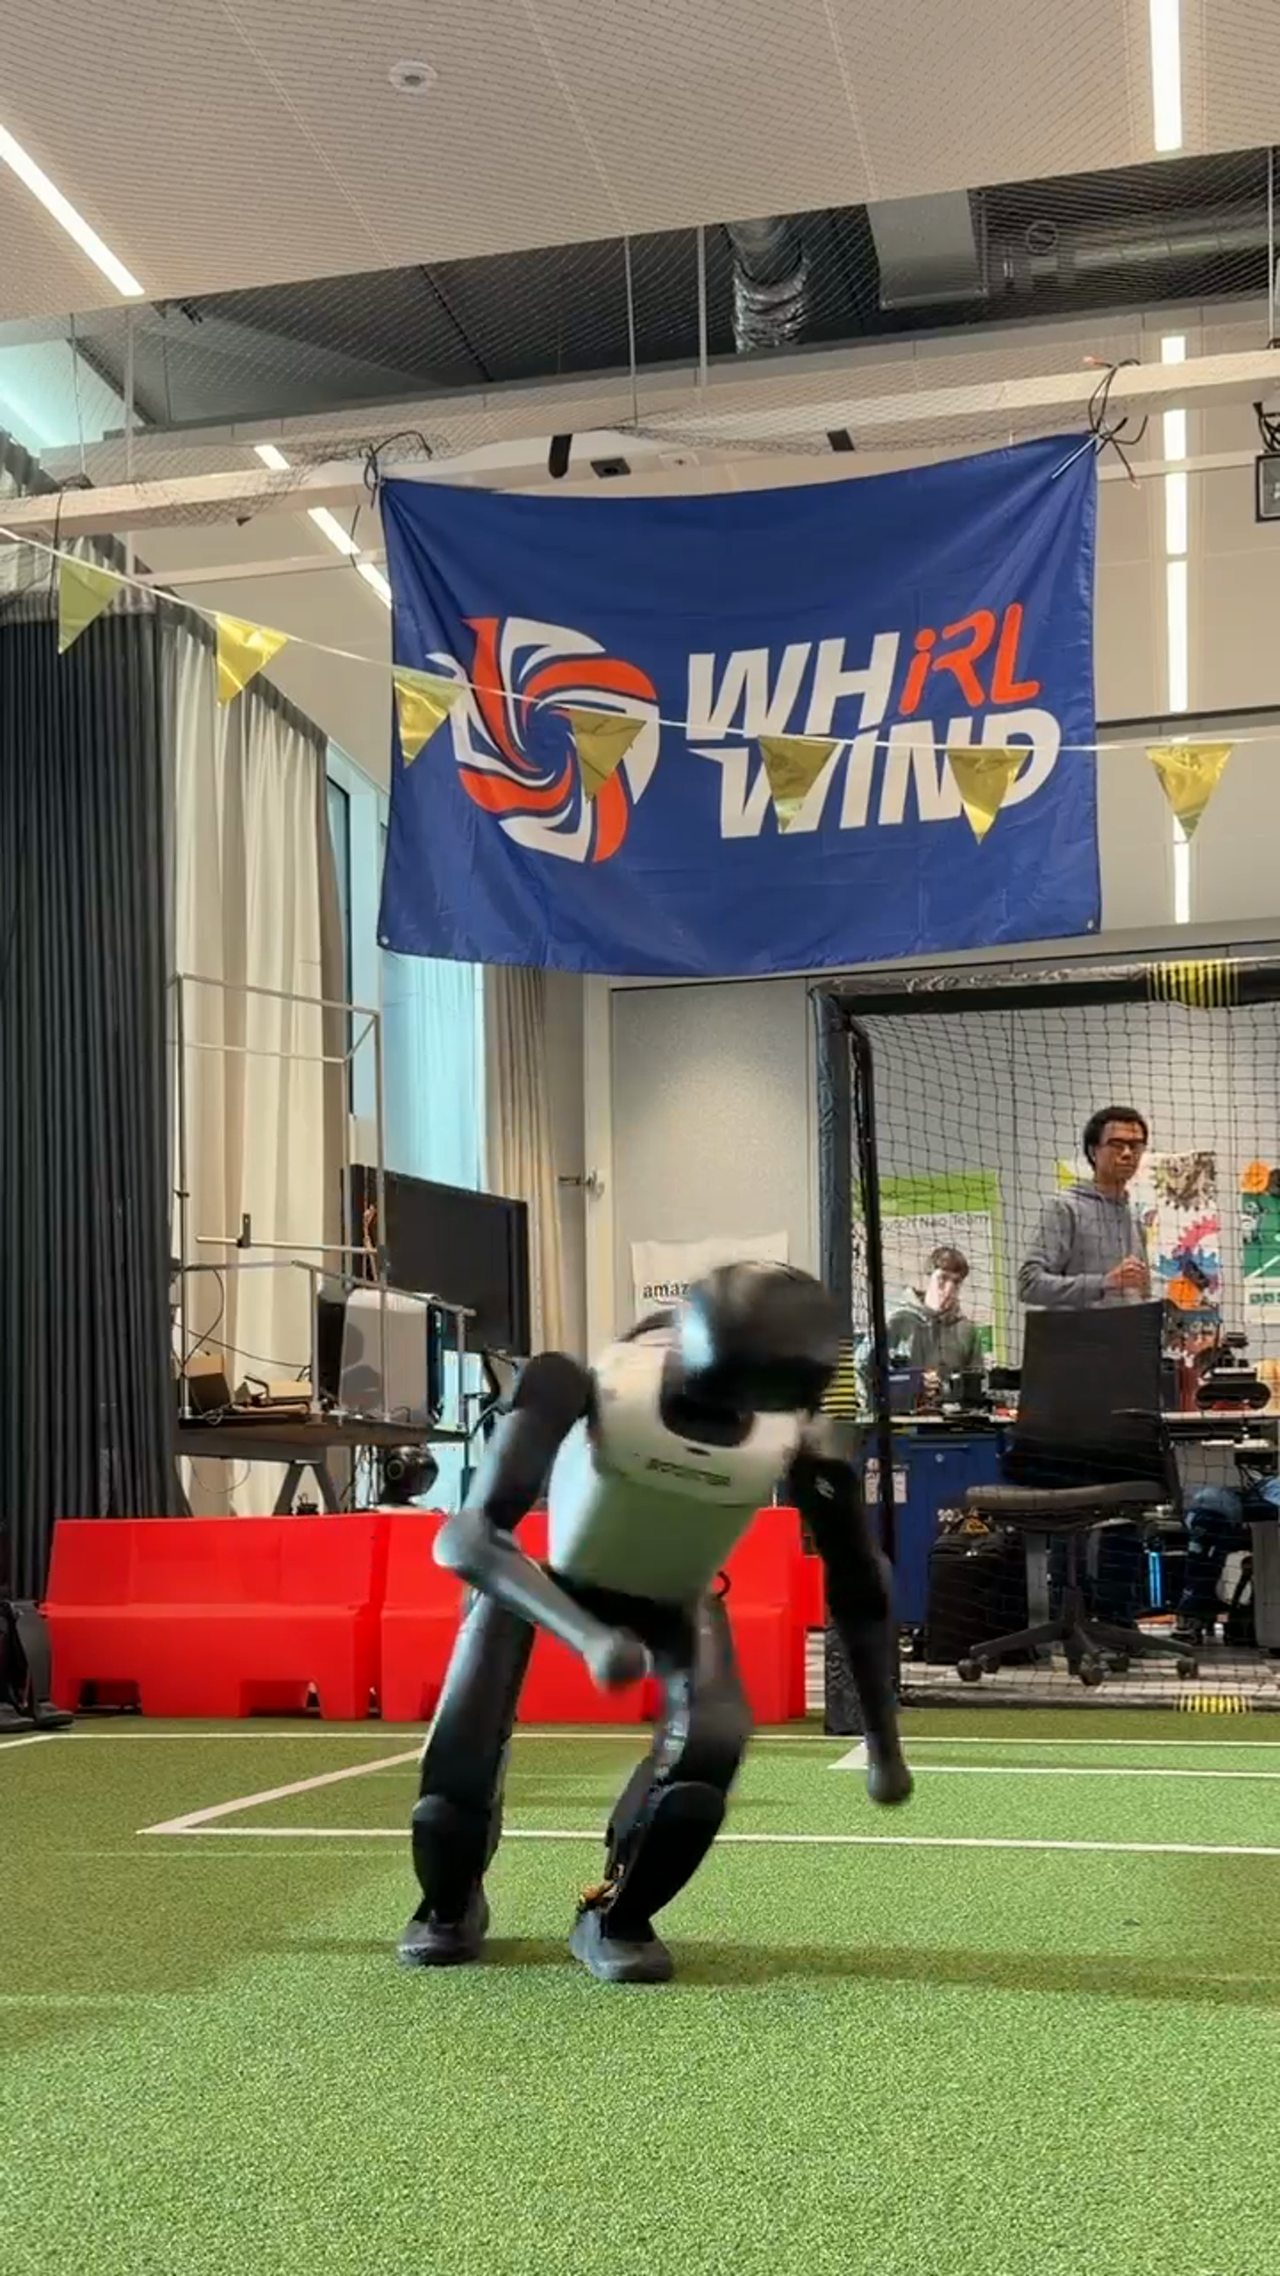
\includegraphics[width=\linewidth]{webster_flip/03.png}
	\end{subfigure}\hfill
	\begin{subfigure}[b]{0.19\textwidth}
		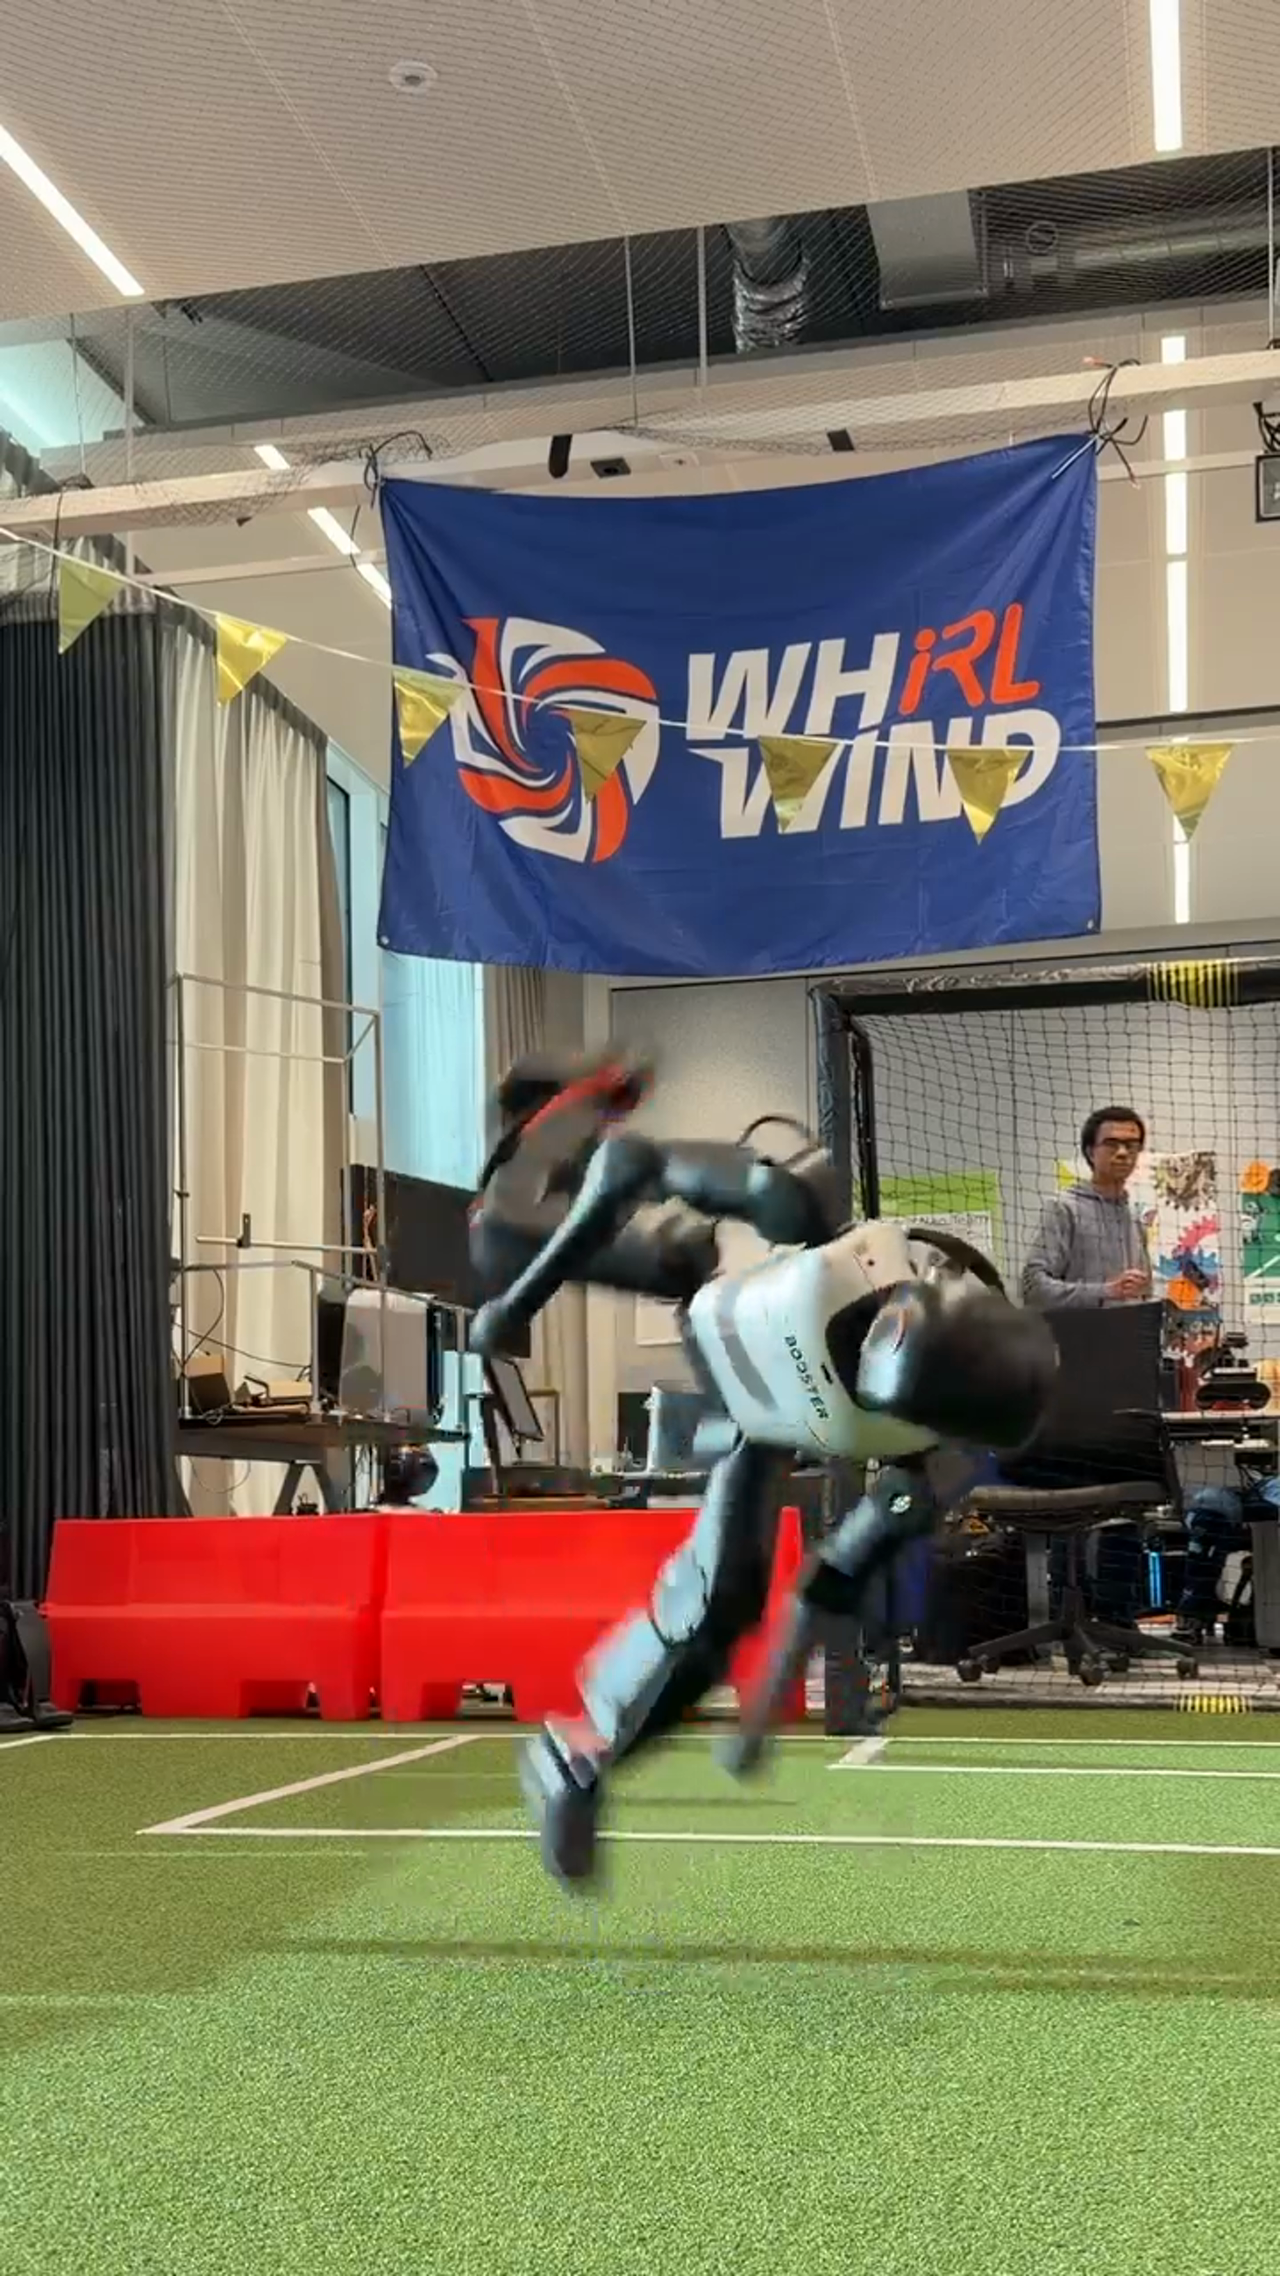
\includegraphics[width=\linewidth]{webster_flip/04.png}
	\end{subfigure}\hfill
	\begin{subfigure}[b]{0.19\textwidth}
		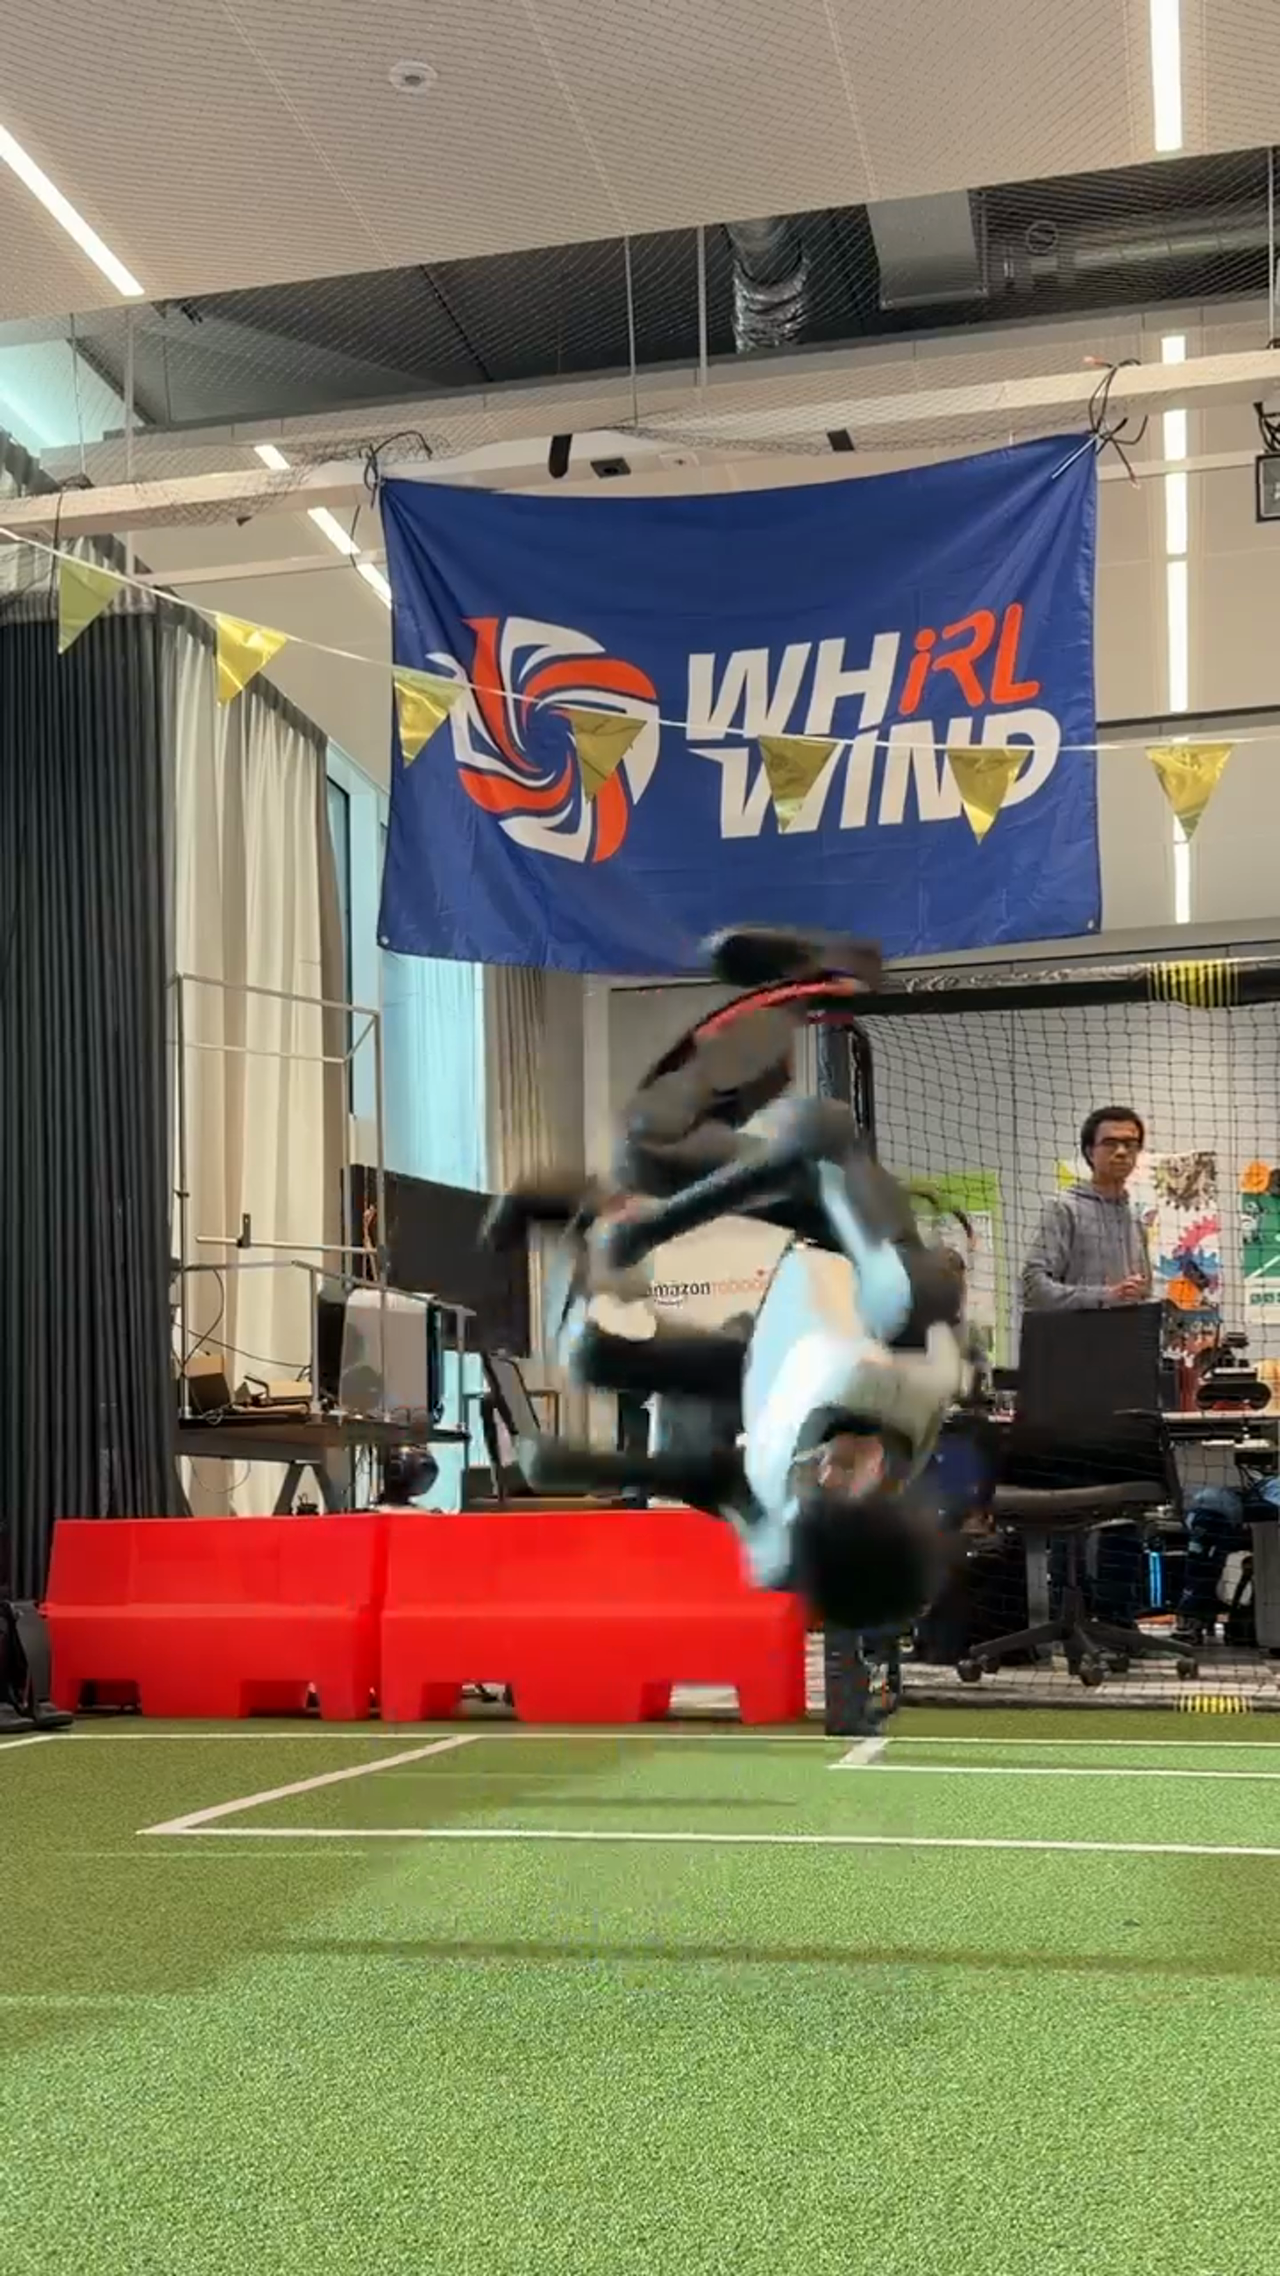
\includegraphics[width=\linewidth]{webster_flip/05.png}
	\end{subfigure}

	\vspace{0.5em} % vertical gap between rows

	\begin{subfigure}[b]{0.19\textwidth}
		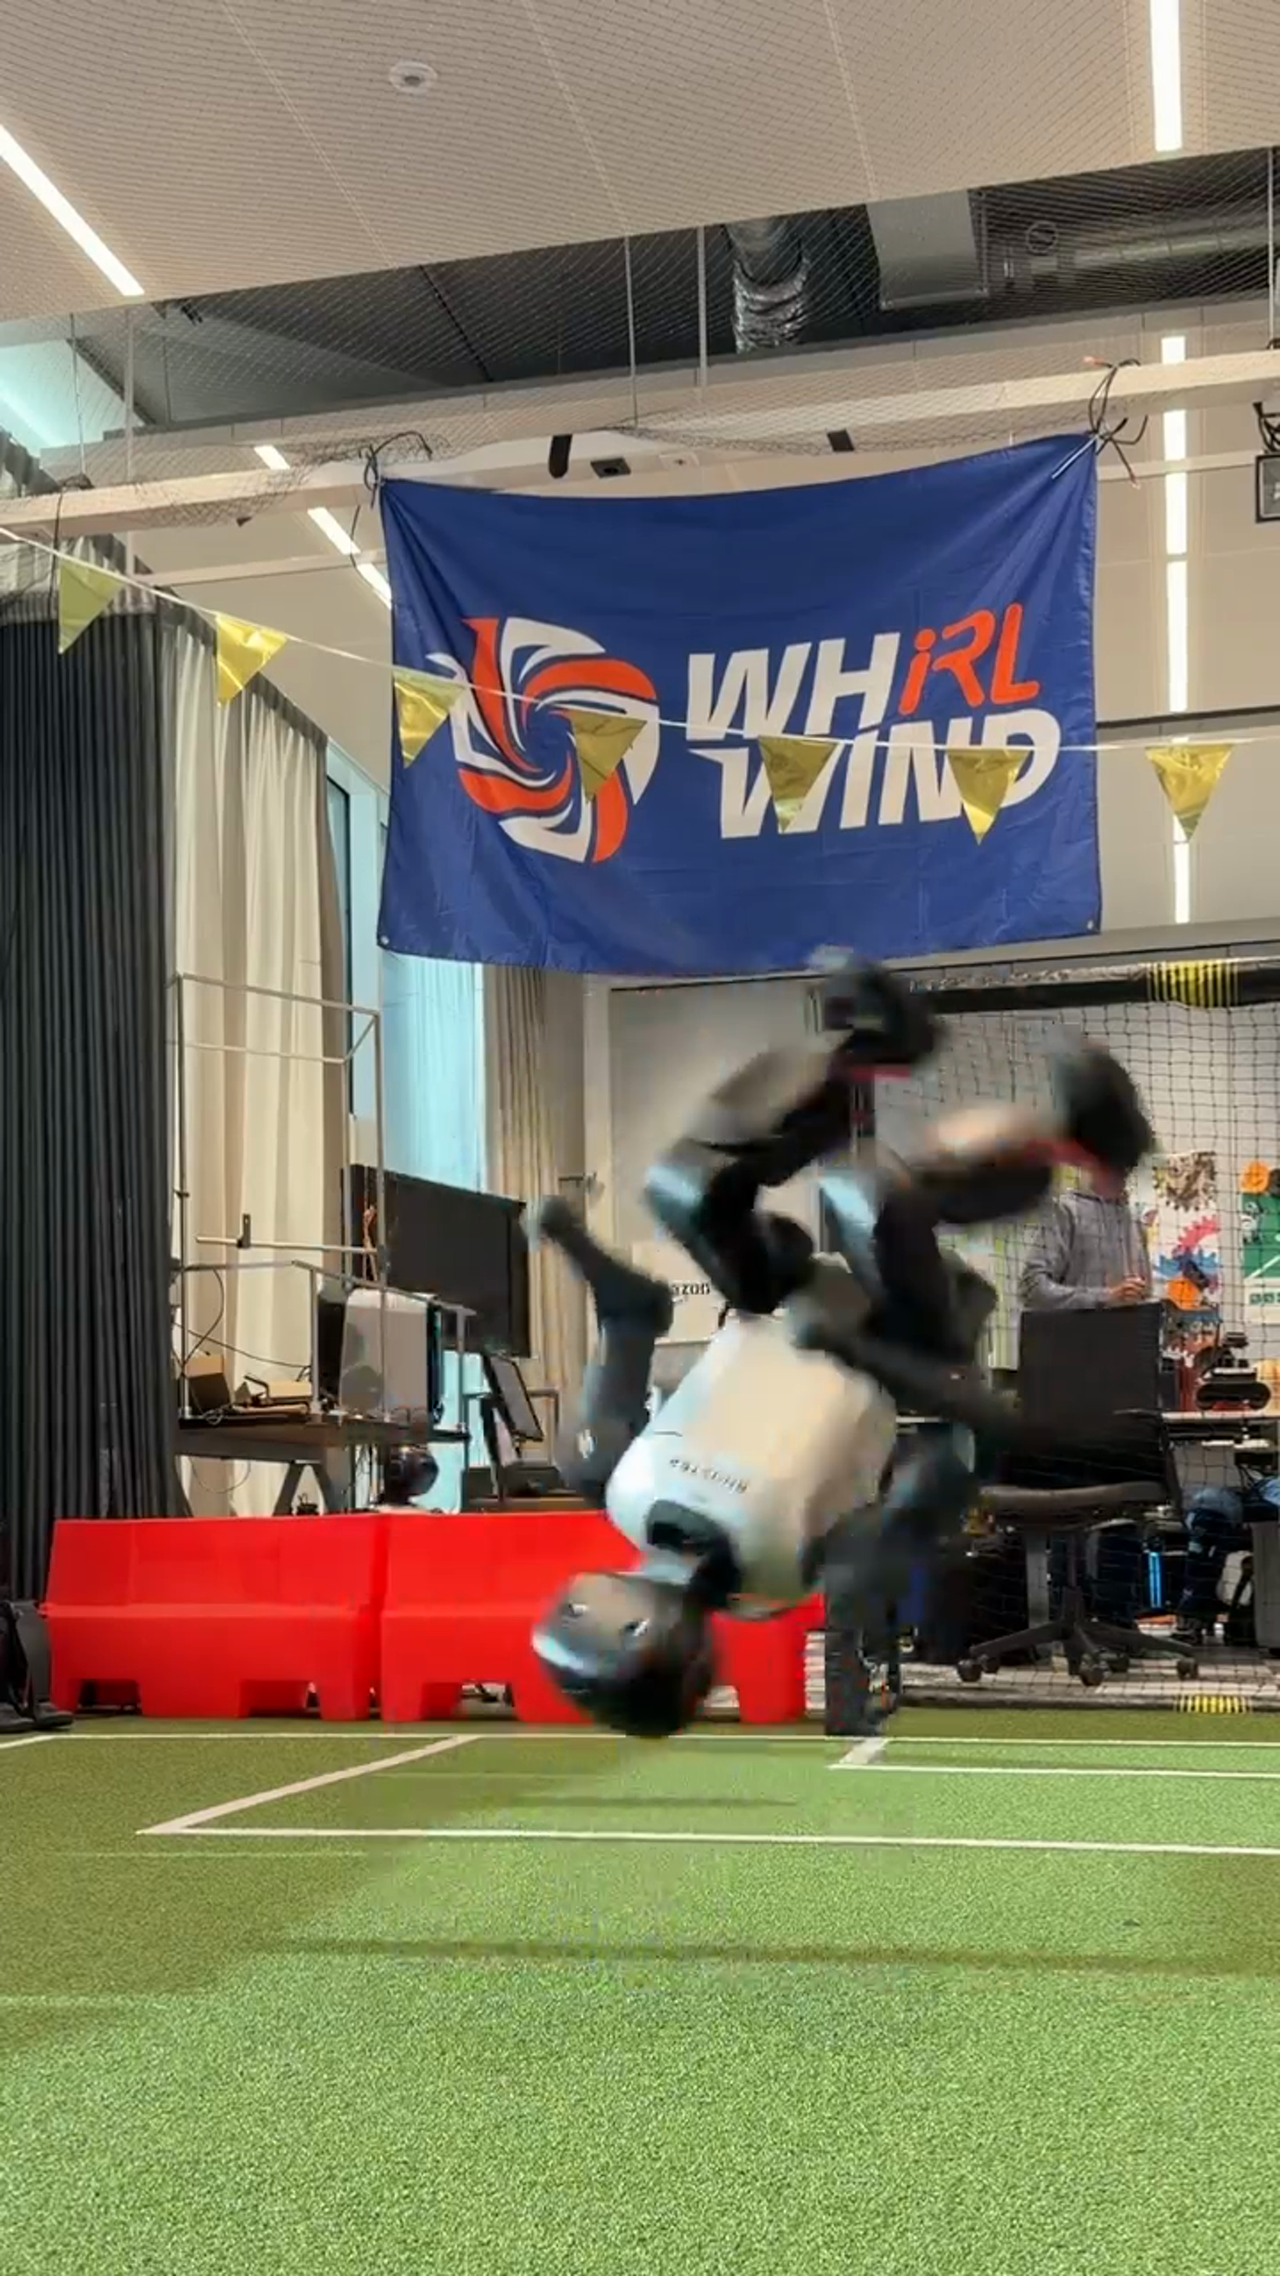
\includegraphics[width=\linewidth]{webster_flip/06.png}
	\end{subfigure}\hfill
	\begin{subfigure}[b]{0.19\textwidth}
		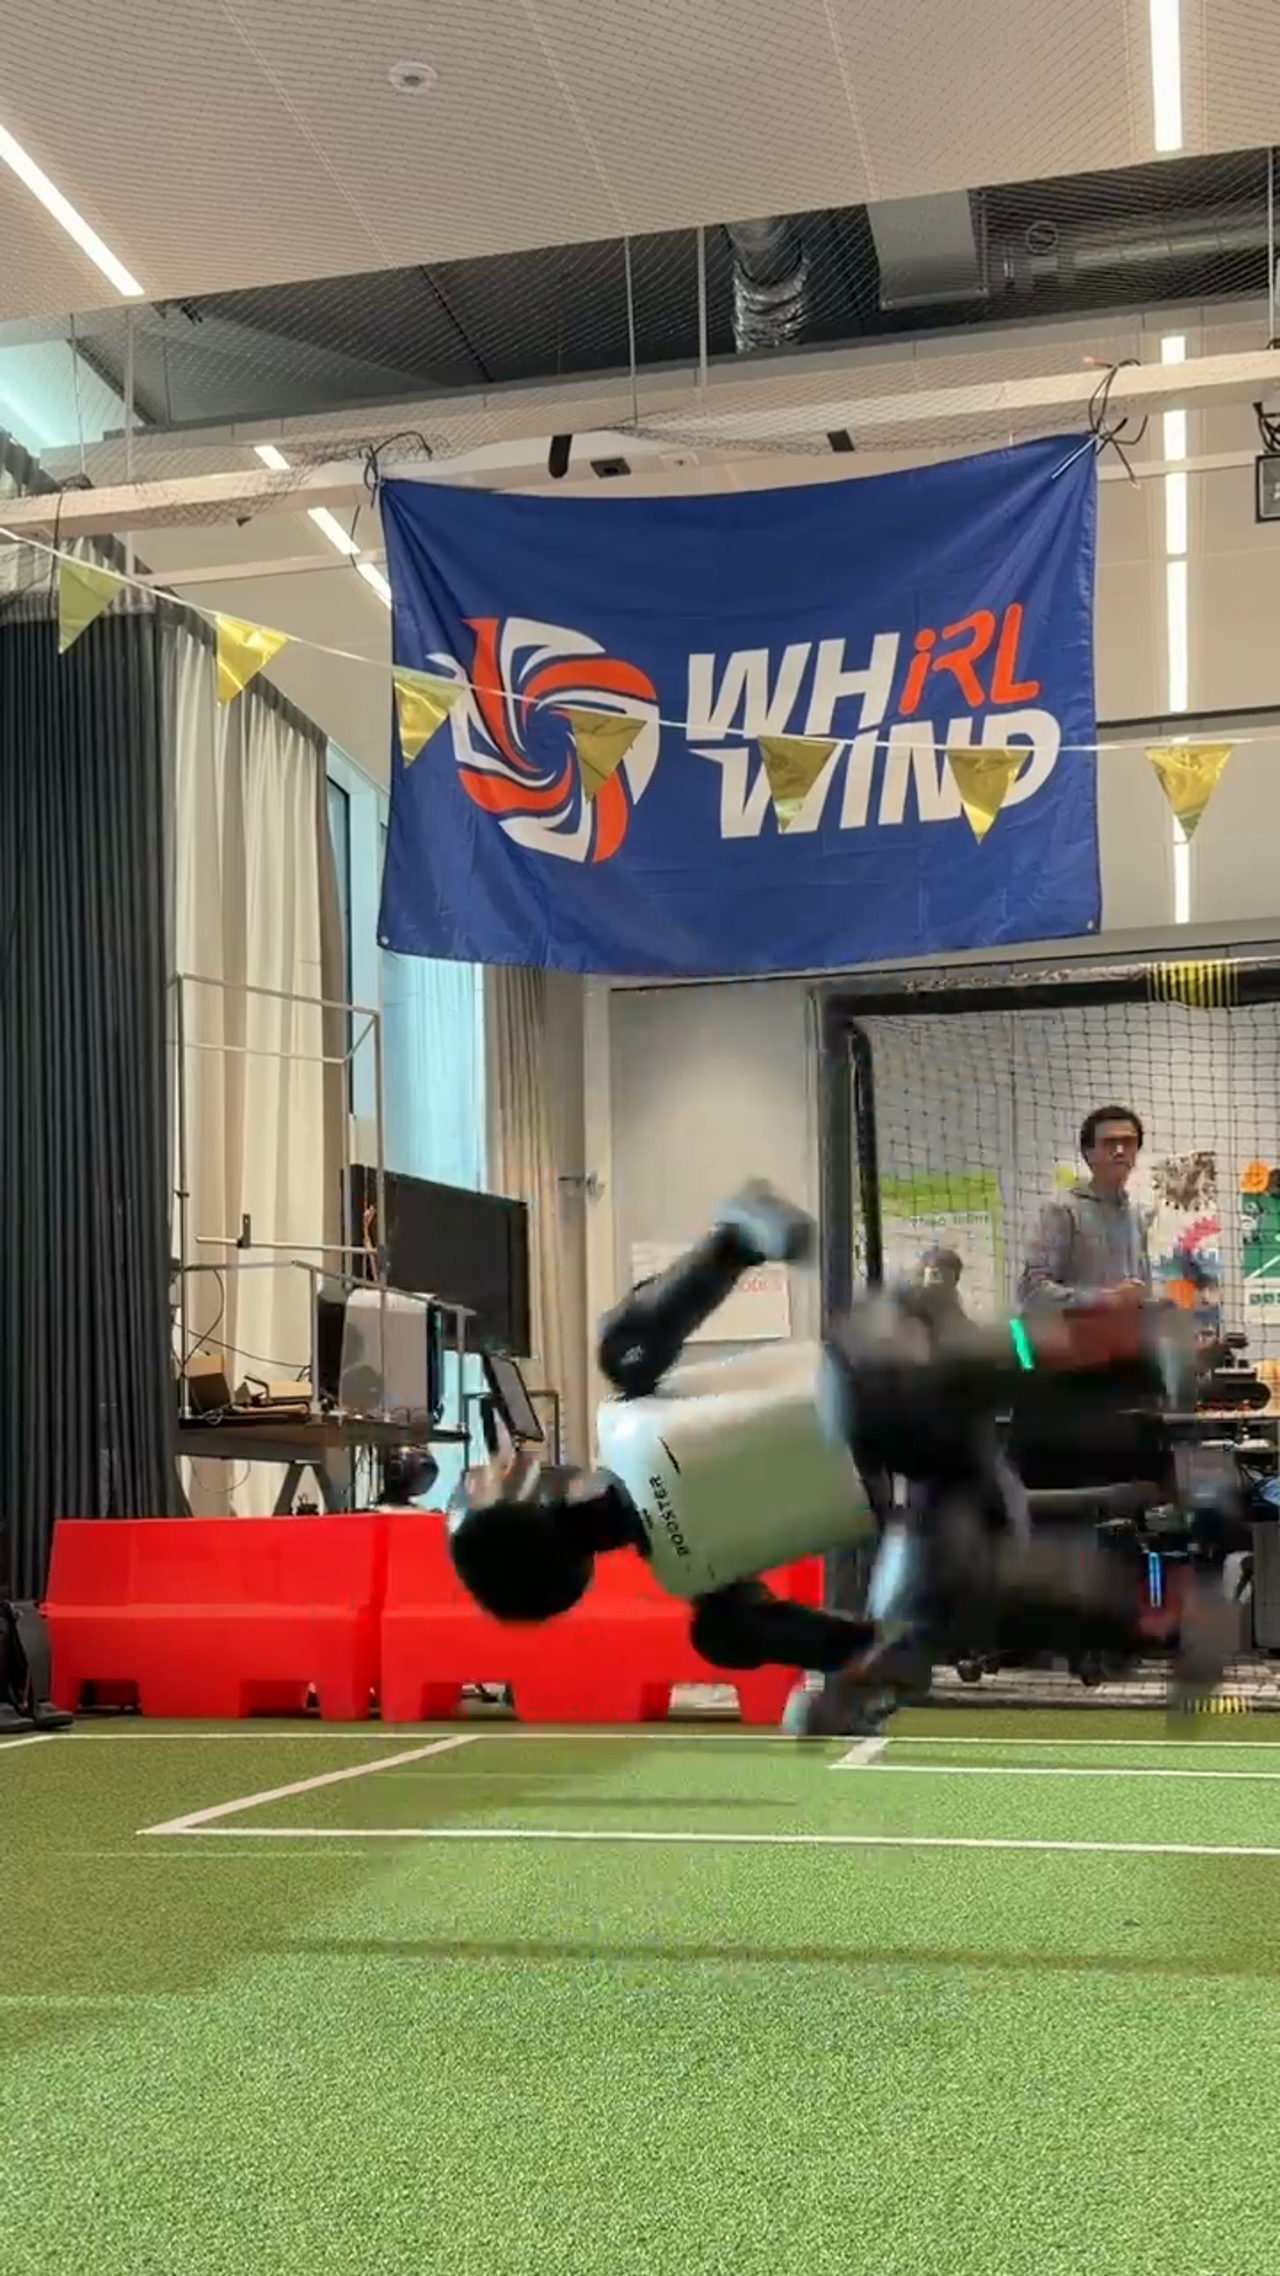
\includegraphics[width=\linewidth]{webster_flip/07.png}
	\end{subfigure}\hfill
	\begin{subfigure}[b]{0.19\textwidth}
		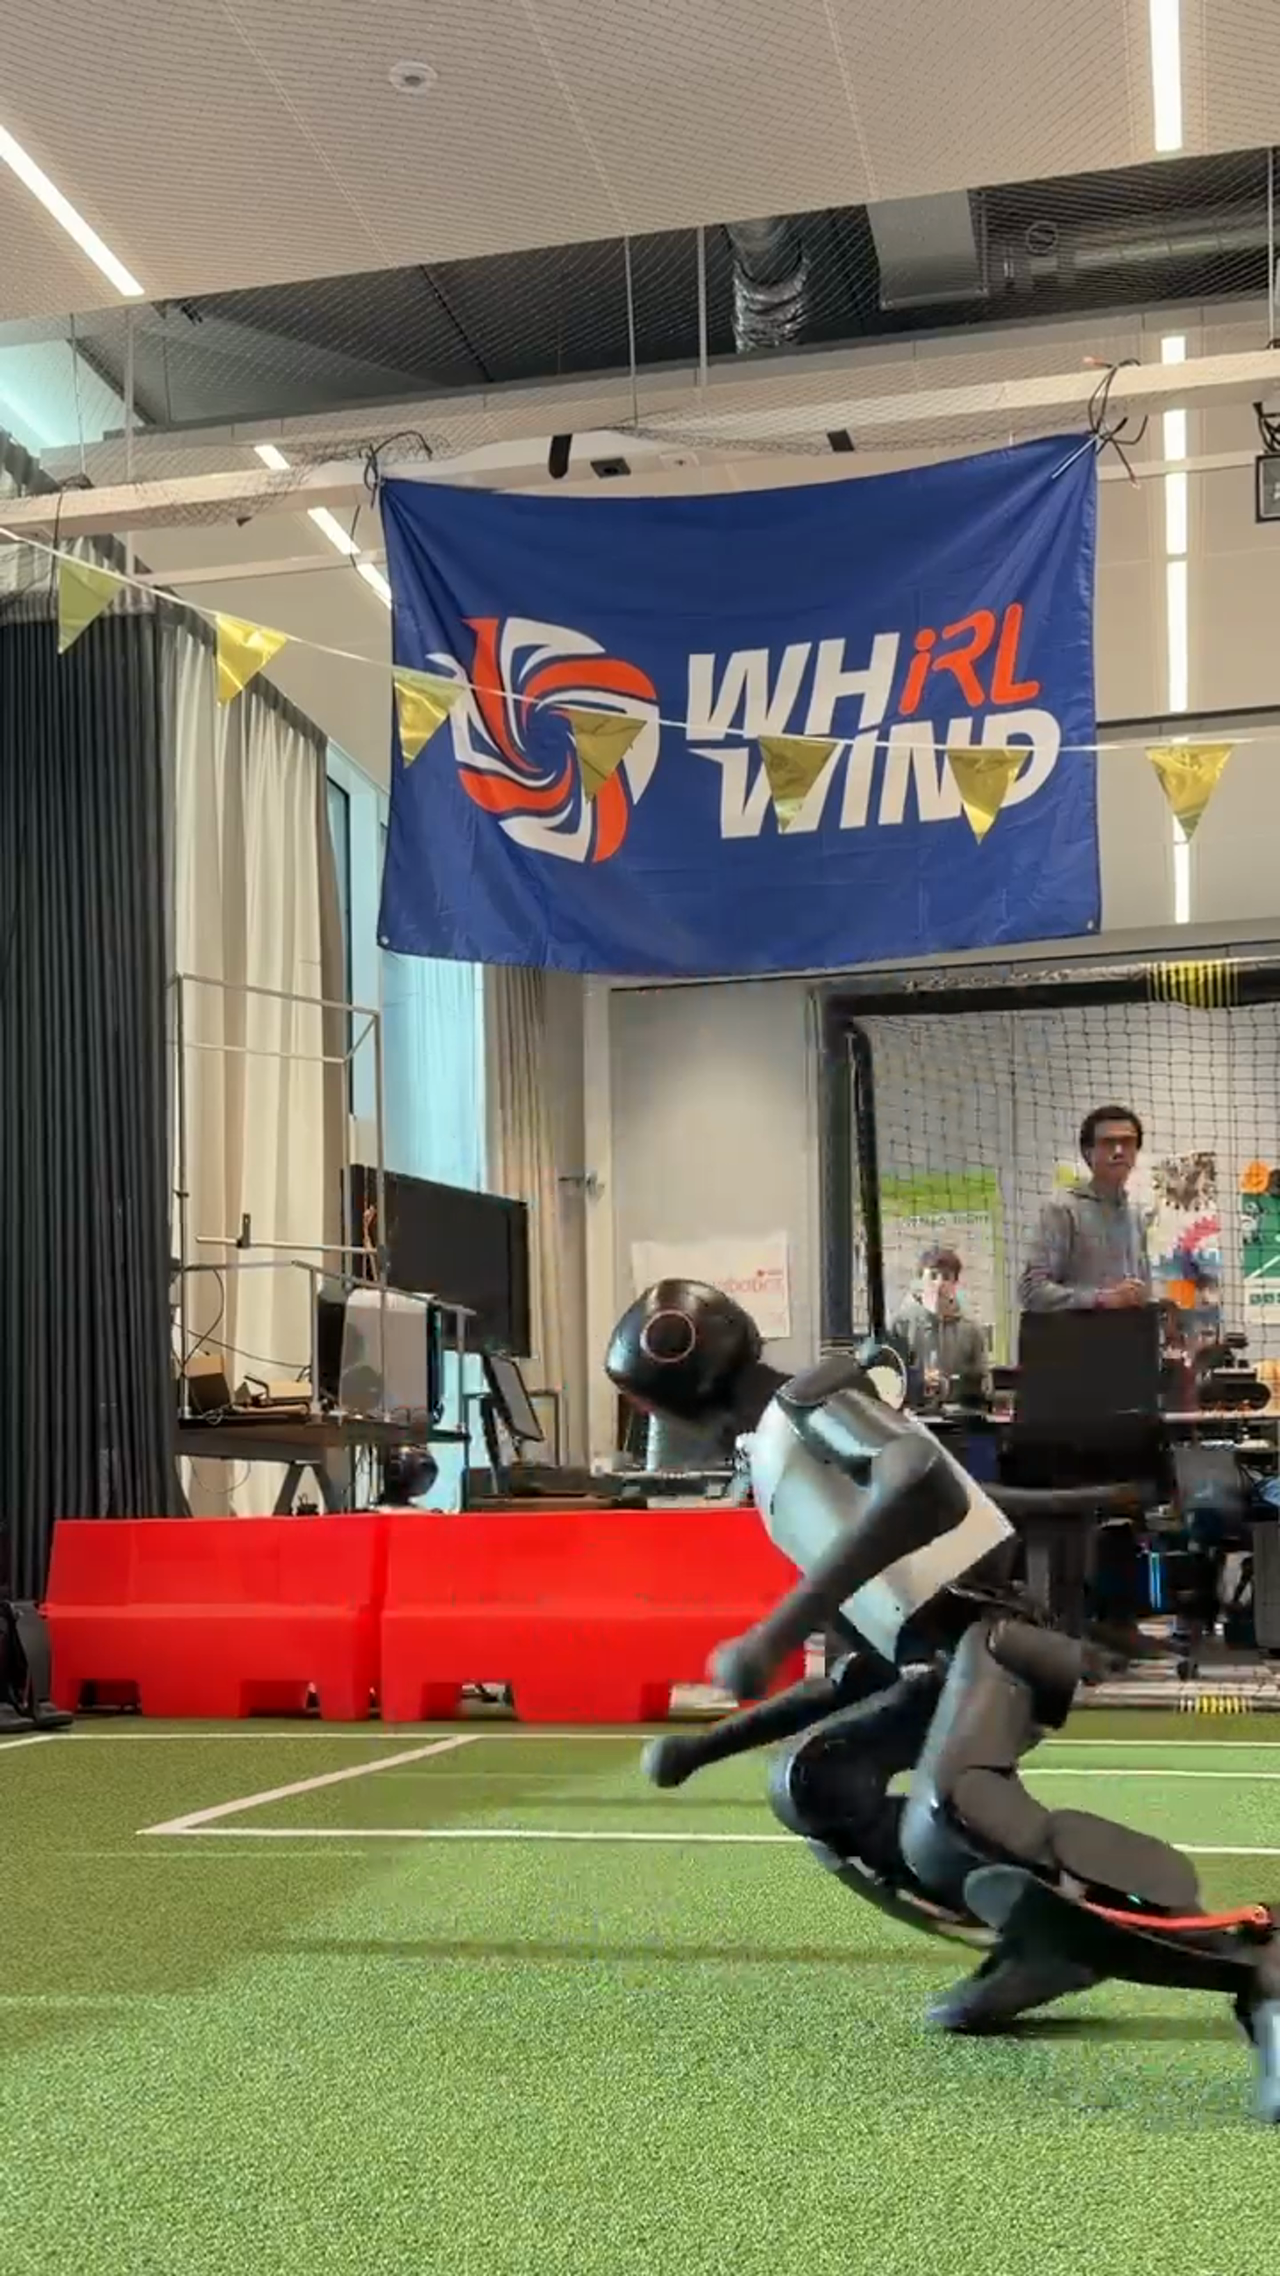
\includegraphics[width=\linewidth]{webster_flip/08.png}
	\end{subfigure}\hfill
	\begin{subfigure}[b]{0.19\textwidth}
		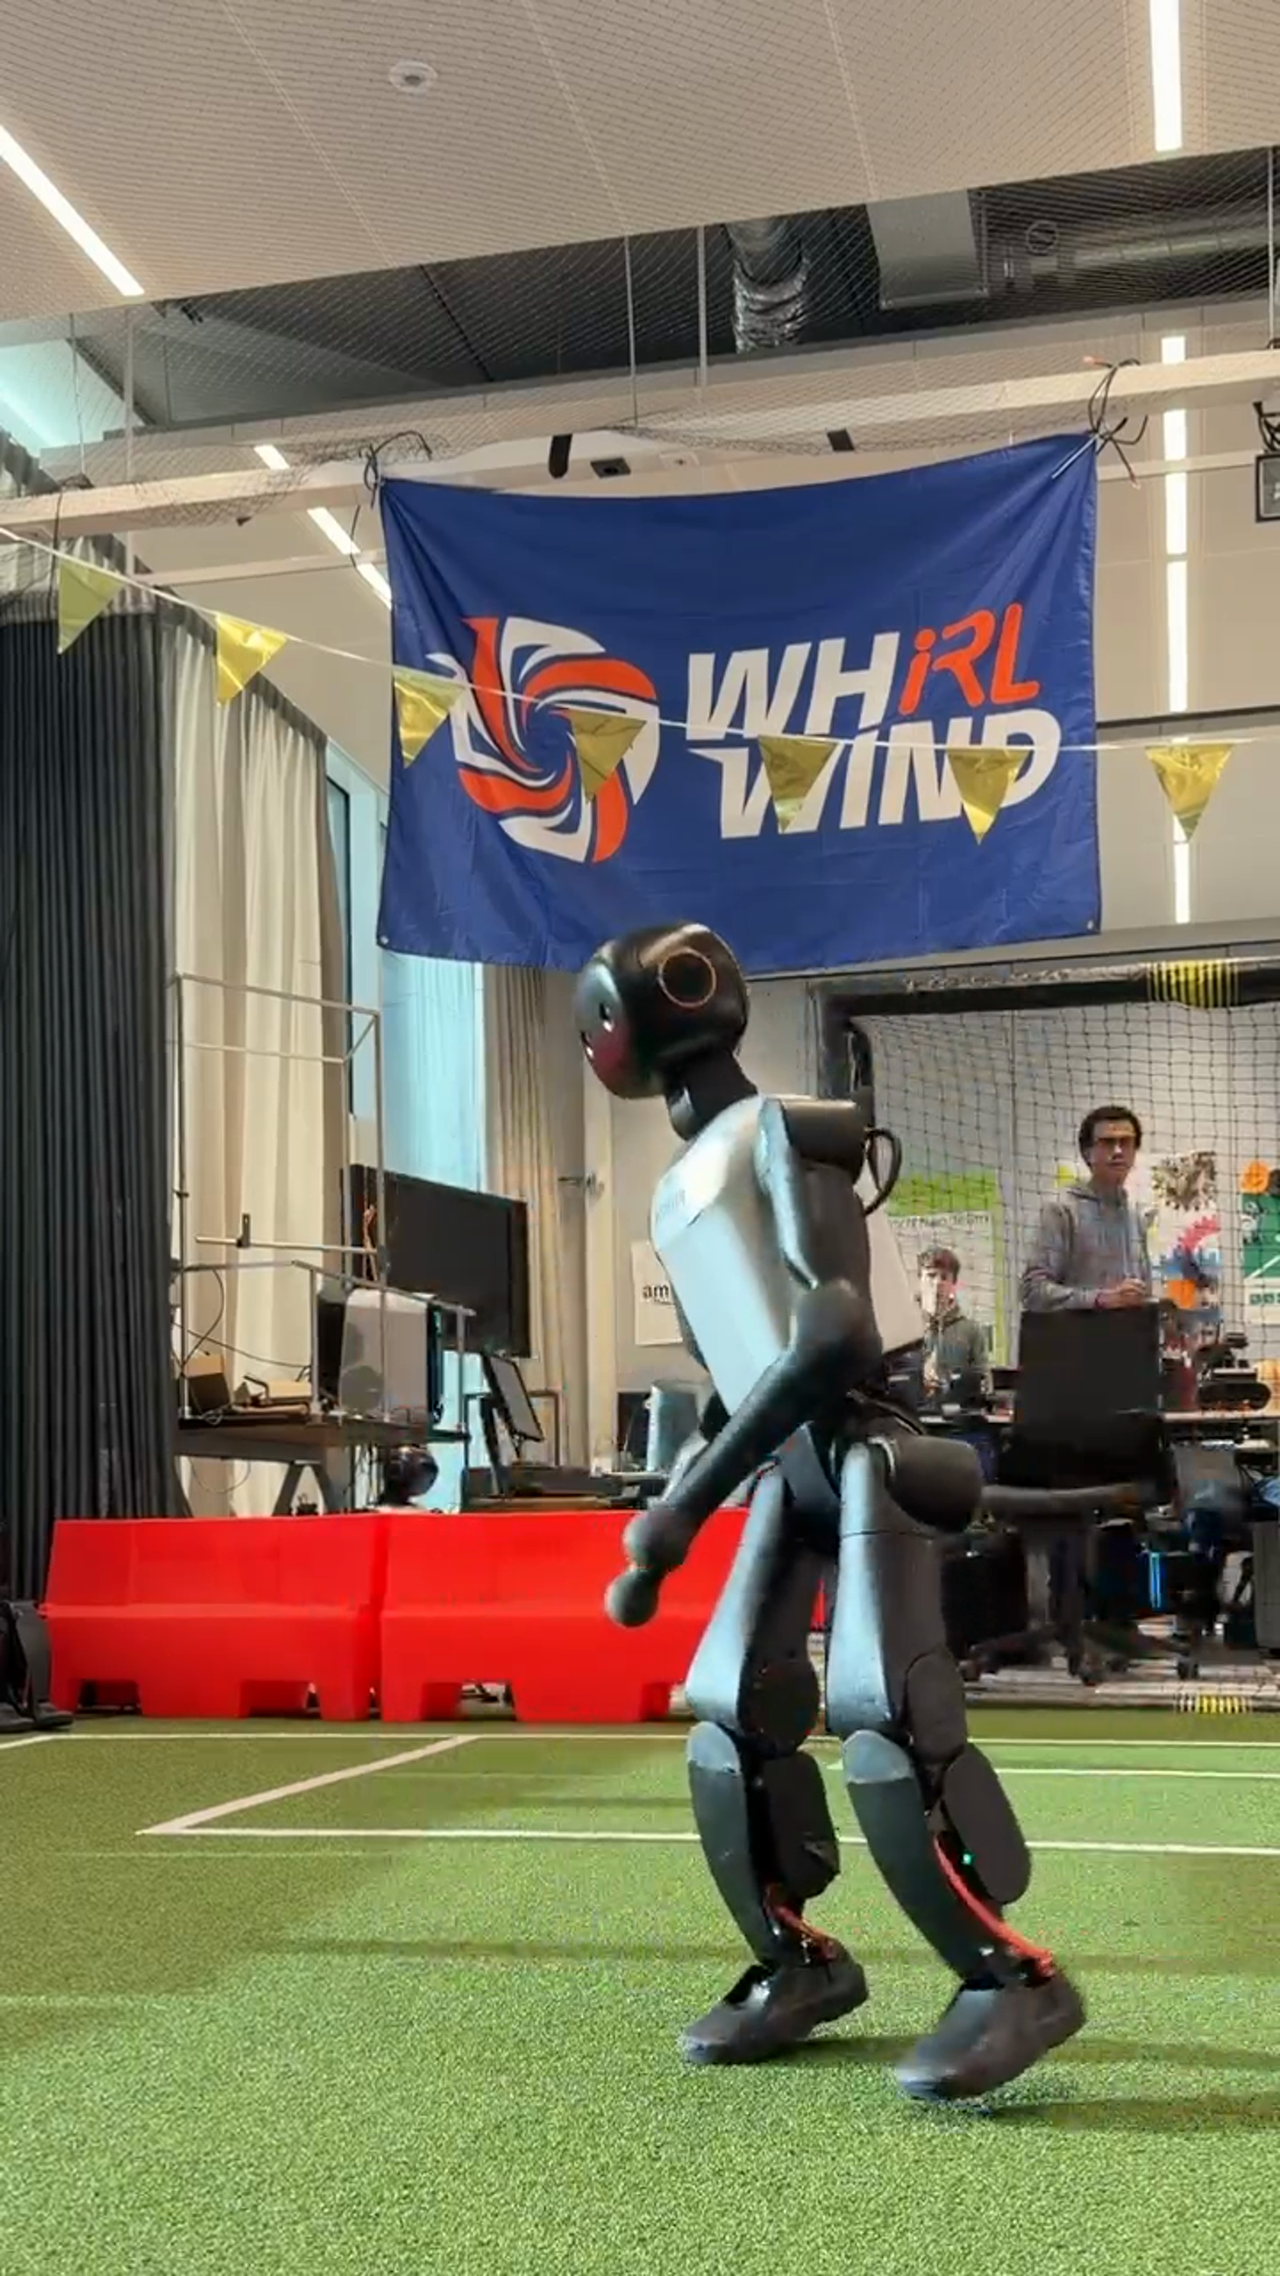
\includegraphics[width=\linewidth]{webster_flip/09.png}
	\end{subfigure}\hfill
	\begin{subfigure}[b]{0.19\textwidth}
		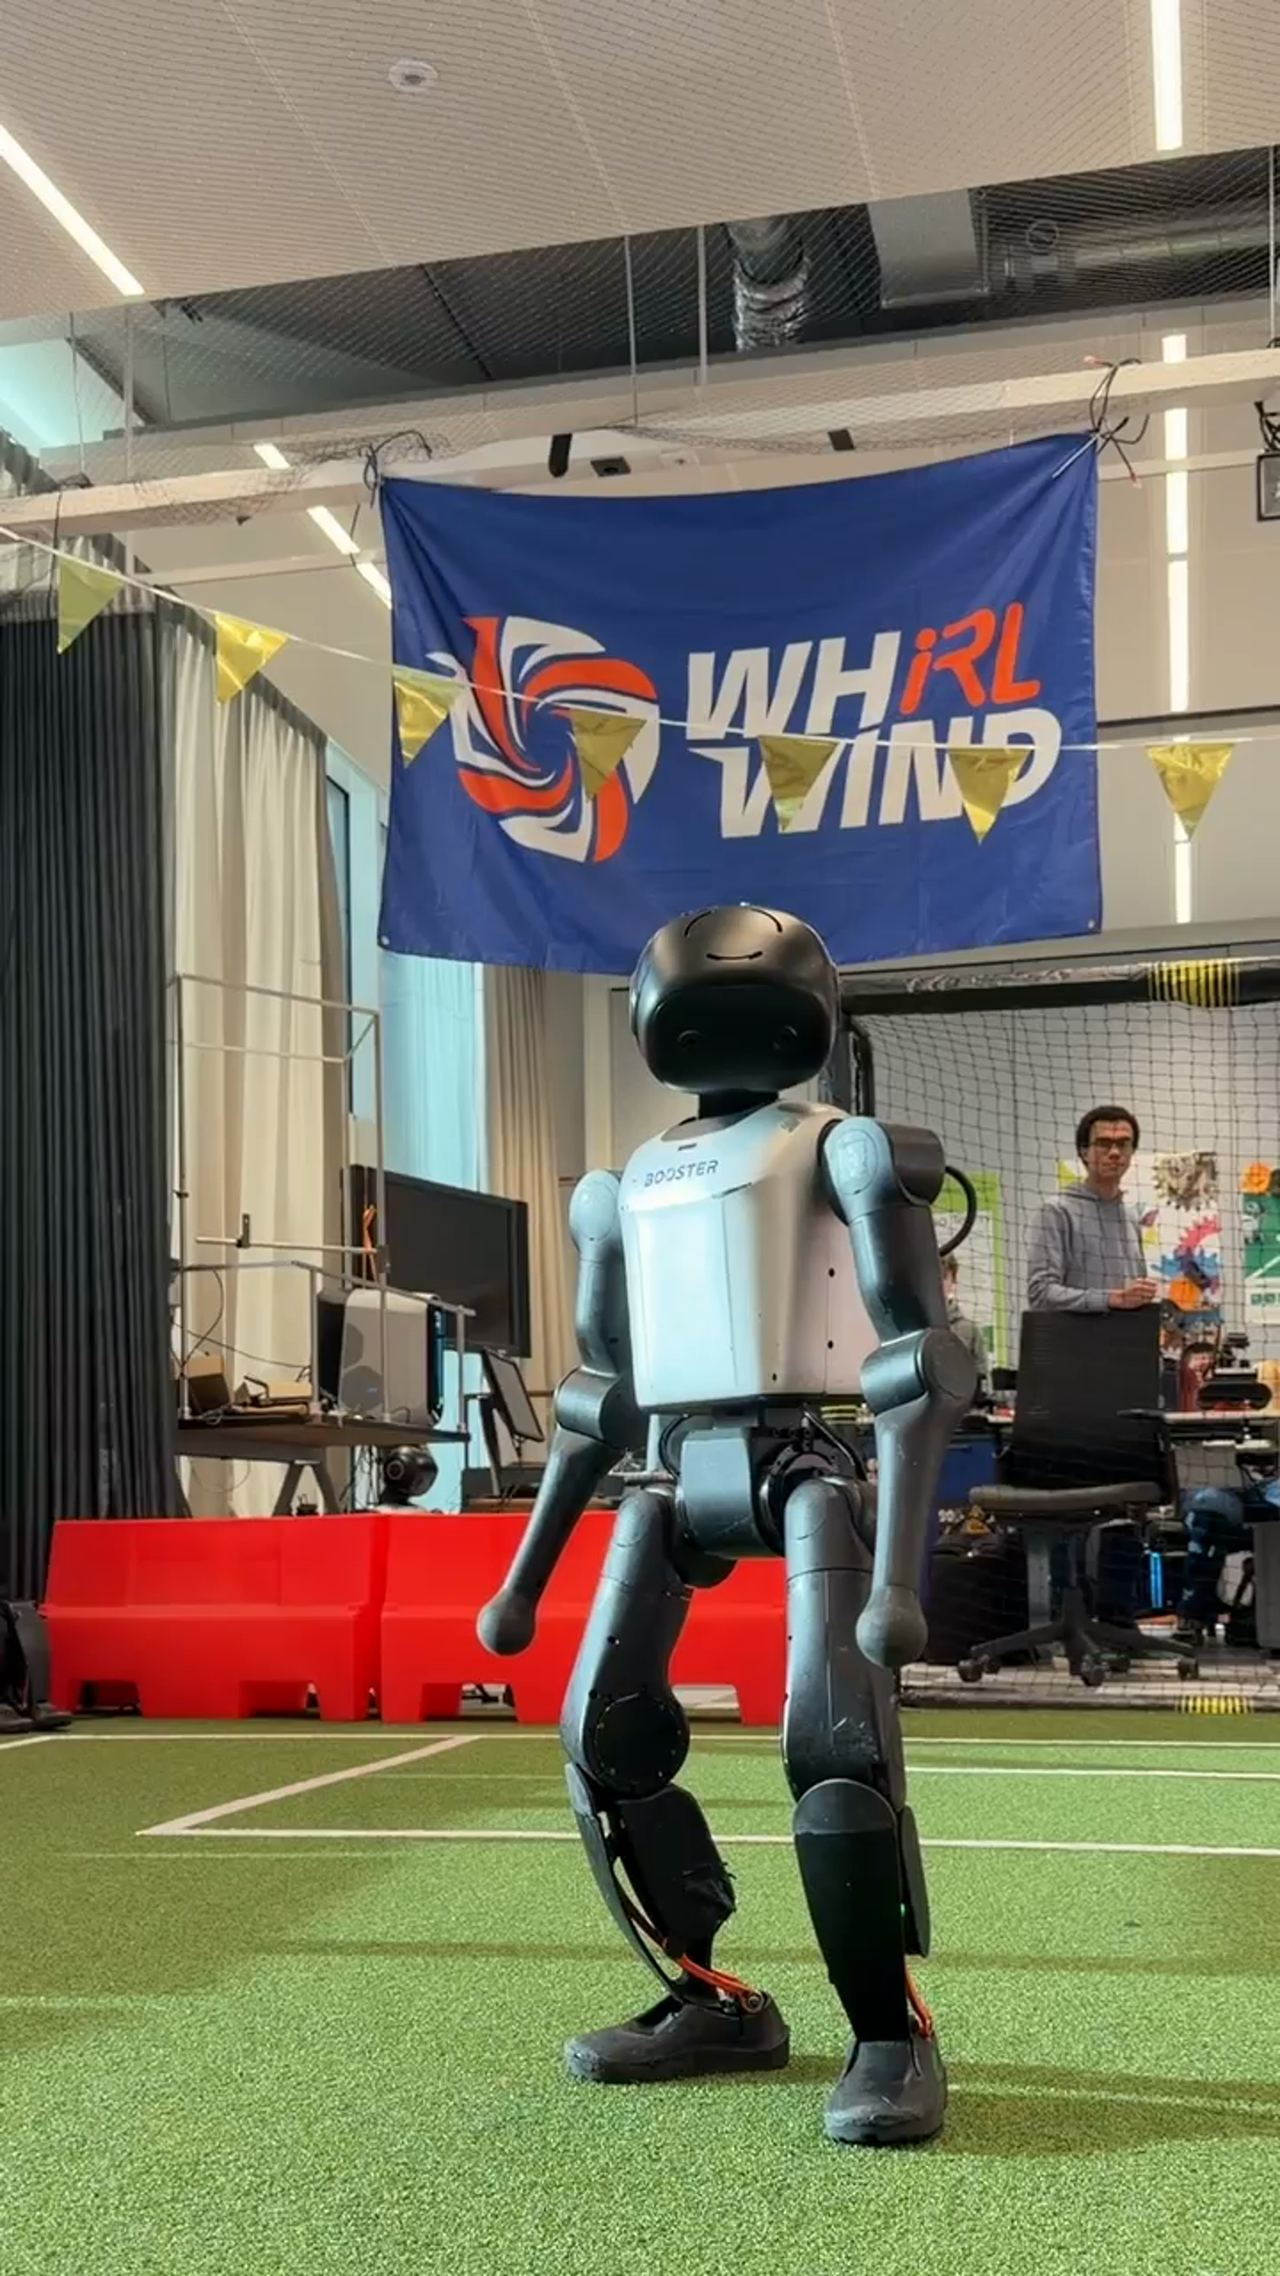
\includegraphics[width=\linewidth]{webster_flip/10.png}
	\end{subfigure}

	\caption{Booster K1 robot doing a webster flip}
	\label{fig:webster_flip}
\end{figure}

During such a motion the robot has to know at every moment how all its joints are bent (angles and trigonometry), where its feet, hands and head are (vectors and matrices), how fast everything rotates and how quickly that changes (derivatives), and how to correct small errors before it falls over (gradients and learning). A modern controller for a motion like this is often a \emph{neural network} that has been trained, and training is nothing but the calculus of this book at work.

\section*{Soccer as a grand challenge}
The flip is only one example of a complex motion. Soccer is full of them: a player has to receive a pass and control the ball, sprint and change direction in a split second, tackle an opponent without fouling, or, as a goalie, jump and catch a shot. All of these demand the same skills as the flip: balance, precise joint control and fast decisions. Soccer therefore combines many hard motion problems in one game, and this is why researchers let robots play it.

The RoboCup federation explains it on its website: RoboCup uses soccer as a long-term challenge to advance robotics and AI research, a ``landmark project'' and a ``standard problem'' on which many teams can compare their ideas\footnote{RoboCup Federation, \emph{Objective}, \url{https://robocup.org/objective}.}. The official long-term goal is:

\begin{quote}
\emph{By the middle of the 21st century, a team of fully autonomous humanoid robot soccer players shall win a soccer game, complying with the official rules of FIFA, against the winner of the most recent World Cup.}
\end{quote}

The organisers call this a grand challenge for the next decades that will not be met in the near future. On the way, the modest goal is to build a robot soccer team that plays like human players.

\section*{What makes it so hard?}
Compared with a game like chess, robot soccer is a much harder problem. The RoboCup objective page names several reasons\footnote{Source of the list and of the research areas below: the same RoboCup objective page.}, and each of them connects to a part of this book:

\begin{center}
\renewcommand{\arraystretch}{1.35}
\begin{tabular}{>{\raggedright\arraybackslash}p{4.3cm}>{\raggedright\arraybackslash}p{4.3cm}>{\raggedright\arraybackslash}p{4.2cm}}
\textbf{Challenge} & \textbf{What it means} & \textbf{Math you will learn}\\ \hline
Dynamic environment & The world keeps changing, unlike a chess board. & Functions, rates of change (Chapters~\ref{ch:functions}--\ref{ch:activation} and \ref{ch:rate}--\ref{ch:integrals})\\
Real-time play & There are no turns: decisions are needed now. & Fast computations with vectors and matrices (Chapters~\ref{ch:vectors}--\ref{ch:rotation})\\
Incomplete information & A robot sees only part of the field. & Coordinates and reference frames (Chapters~\ref{ch:coordinates}--\ref{ch:frames})\\
Raw sensor data & Cameras and sensors deliver numbers, not ``ball at $(4,5)$''. & Geometry, distances, vectors (Chapters~\ref{ch:coordinates}--\ref{ch:rotation})\\
Distributed control & Every robot decides for itself. & Neural networks (Chapter~\ref{ch:nn})\\
Motor control and learning & Walking, kicking and flipping need precise motions. & Trigonometry, matrices, gradient descent (Chapters~\ref{ch:coordinates}--\ref{ch:integrals})\\
\end{tabular}
\end{center}

The same page lists the research areas that RoboCup brings together: sensor fusion, reactive behaviour, multi-agent systems, real-time planning, learning and motor control. All of them are built on the topics you are about to study.

\begin{keyidea}[Your goal]
By the end of this book you will understand the mathematics behind a neural network that learns, and behind the geometry that tells a robot where it is and how to move. This is the foundation on which a robot, one day, can play like a champion.
\end{keyidea}

\chapter*{What you need for this course}
\markboth{Course requirements}{Course requirements}
\addcontentsline{toc}{chapter}{What you need for this course}

To follow the course and to try out the ideas of this book on a real machine, you need the following.

\begin{keyidea}[Requirements]
\begin{itemize}[nosep]
  \item \textbf{A laptop with Ubuntu 26.04.} It is used for the problems marked with \texttt{[code]}, for plotting and for programming the examples of this book.
  \item \textbf{A Booster K1 robot.} The humanoid robot from the title page and from the webster flip in the Motivation chapter. You will use it to test what you have learned on a real robot.
\end{itemize}
\end{keyidea}

\textbf{Before the first lesson.} Make sure that the laptop starts and that you can log in to your Ubuntu account. Check that the robot is charged and that you know who is responsible for it in your group.

\textbf{Working in groups.} If robots or laptops are shared, agree in your group who is using which device and when, so that everybody can try the code and the robot.


\mainmatter

% =====================================================================
\part{Mathematical Foundations}\label{part:math}
\block{Foundations: Functions, Algebra and Sums}
\includechapter{part01_math/block1_foundations/ch01_functions_and_graphs}
\includechapter{part01_math/block1_foundations/ch02_algebra_essentials}
\includechapter{part01_math/block1_foundations/ch03_summation_notation}
\includechapter{part01_math/block1_foundations/ch04_activation_functions}
\block{Geometry and Trigonometry}
\includechapter{part01_math/block2_geometry_trigonometry/ch05_coordinate_systems}
\includechapter{part01_math/block2_geometry_trigonometry/ch06_angles_and_trigonometry}
\includechapter{part01_math/block2_geometry_trigonometry/ch07_pythagoras_and_distance}
\includechapter{part01_math/block2_geometry_trigonometry/ch08_reference_frames}
\block{Vectors and Matrices}
\includechapter{part01_math/block3_vectors_matrices/ch09_vectors}
\includechapter{part01_math/block3_vectors_matrices/ch10_dot_product}
\includechapter{part01_math/block3_vectors_matrices/ch11_matrices}
\includechapter{part01_math/block3_vectors_matrices/ch12_rotation_and_translation}
\block{Calculus: How a Network Learns}
\includechapter{part01_math/block4_calculus/ch13_rate_of_change}
\includechapter{part01_math/block4_calculus/ch14_the_derivative}
\includechapter{part01_math/block4_calculus/ch15_derivative_rules}
\includechapter{part01_math/block4_calculus/ch16_chain_rule}
\includechapter{part01_math/block4_calculus/ch17_key_functions}
\includechapter{part01_math/block4_calculus/ch18_minima_and_maxima}
\includechapter{part01_math/block4_calculus/ch19_partial_derivatives_gradient}
\includechapter{part01_math/block4_calculus/ch20_gradient_descent}
\includechapter{part01_math/block4_calculus/ch21_numerical_derivatives}
\includechapter{part01_math/block4_calculus/ch22_integrals}
\block{A Tiny Neural Network}
\includechapter{part01_math/block5_neural_network/ch23_a_tiny_neural_network}
\block{Probability and Statistics (planned)}
\includeplanned{part01_math/block6_probability/01_probability_basics}
\includeplanned{part01_math/block6_probability/02_statistics_and_the_normal_distribution}

% =====================================================================
\part{Linux}\label{part:linux}
\includeplanned{part02_linux/01_login_shell_files_and_permissions}
\includeplanned{part02_linux/02_remote_work_with_ssh}
\includeplanned{part02_linux/03_packages_and_environments}
\includeplanned{part02_linux/04_processes_systemd_and_logs}
\includeplanned{part02_linux/05_networking_from_the_command_line}
\includeplanned{part02_linux/06_git_and_version_control}

% =====================================================================
\part{Python Programming}\label{part:python}
\includeplanned{part03_python/01_python_basics}
\includeplanned{part03_python/02_collections_and_files}
\includeplanned{part03_python/03_numpy_and_matplotlib}
\includeplanned{part03_python/04_classes_and_modules}
\includeplanned{part03_python/05_images_and_video_with_opencv}
\includeplanned{part03_python/06_testing_and_debugging}

% =====================================================================
\part{Hardware}\label{part:hardware}
\includeplanned{part04_hardware/01_how_a_computer_works}
\includeplanned{part04_hardware/02_networking}
\includeplanned{part04_hardware/03_sensors}
\includeplanned{part04_hardware/04_microphones_and_sound}
\includeplanned{part04_hardware/05_motors}
\includeplanned{part04_hardware/06_modern_robot_actuators}
\includeplanned{part04_hardware/07_power_and_safety}

% =====================================================================
\part{ROS 2}\label{part:ros}
\includeplanned{part05_ros2/01_ros_2_concepts}
\includeplanned{part05_ros2/02_launch_files_and_parameters}
\includeplanned{part05_ros2/03_coordinate_frames_with_tf2}
\includeplanned{part05_ros2/04_logging_replay_and_visualisation}
\includeplanned{part05_ros2/05_writing_your_own_nodes}

% =====================================================================
\part{Artificial Intelligence}\label{part:ai}
\includeplanned{part06_ai/01_what_can_ai_do_an_overview_of_tasks}
\includeplanned{part06_ai/02_preparing_data_for_neural_networks}
\includeplanned{part06_ai/03_convolutional_networks}
\includeplanned{part06_ai/04_object_detection_and_yolo}
\includeplanned{part06_ai/05_training_vision_models_effectively}
\includeplanned{part06_ai/06_running_models_on_the_robot}
\includeplanned{part06_ai/07_language_models_and_llms}

% =====================================================================
\part{Reinforcement Learning}\label{part:rl}
\includechapter{part07_rl/01_agent_environment_and_reward}
\includechapter{part07_rl/02_markov_decision_processes_and_value_func}
\includechapter{part07_rl/03_q_learning_and_policy_gradients}
\includechapter{part07_rl/04_deep_rl_and_ppo}
\includechapter{part07_rl/05_reward_design}
\includechapter{part07_rl/06_simulation_and_sim_to_real}

% =====================================================================
\part{Rust Programming}\label{part:rust}
\includeplanned{part08_rust/01_rust_basics}
\includeplanned{part08_rust/02_why_rust_for_robots}
\includeplanned{part08_rust/03_rust_and_ros_2}

% =====================================================================
\part{Motions for the Booster K1}\label{part:k1}
\includeplanned{part09_booster_k1/01_simulators_and_your_first_simulation}
\includeplanned{part09_booster_k1/02_the_booster_k1}
\includeplanned{part09_booster_k1/03_kinematics_of_the_k1}
\includeplanned{part09_booster_k1/04_standing_balance_and_walking}
\includeplanned{part09_booster_k1/05_training_motions_in_simulation}
\includeplanned{part09_booster_k1/06_from_simulation_to_the_real_k1}

% =====================================================================
\part{Control, State Estimation and Perception}\label{part:control}
\includeplanned{part10_control_perception/01_pid_control}
\includeplanned{part10_control_perception/02_balance_and_centre_of_mass}
\includeplanned{part10_control_perception/03_state_estimation_and_the_kalman_filter}
\includeplanned{part10_control_perception/04_sensor_fusion_with_the_imu}
\includeplanned{part10_control_perception/05_localisation_on_the_field}
\includeplanned{part10_control_perception/06_the_perception_pipeline}

% =====================================================================
\part{RoboCup}\label{part:robocup}
\includeplanned{part11_robocup/01_robocup_leagues_rules_and_game_flow}
\includeplanned{part11_robocup/02_behaviour_and_team_play}
\includeplanned{part11_robocup/03_engineering_practice}
\includeplanned{part11_robocup/04_real_time_and_reliability}
\includeplanned{part11_robocup/05_preparing_for_a_tournament}

% =====================================================================
\part{Bonus: Video Analysis}\label{part:bonus}
\includeplanned{part12_bonus_video_analysis/01_analysing_match_video}

\ifdefstring{\answermode}{back}{%
  \backmatter
  \chapter*{Answers to the Practice Problems}
  \markboth{Answers}{Answers}
  \addcontentsline{toc}{chapter}{Answers to the Practice Problems}
  \collectedanswers
}{}

\end{document}
